% Sezione 4
\section{Risultati Sperimentali}
\label{sec:result}
Nella seguente sezione mostriamo i risultati ottenuti dalle nostre sperimentazioni e le
comparazioni con il modello di riferimento in \cite{lyu2018deep}.
% 4.1
\subsection{Valutazione Classificazione}
Usando la 10-fold cross validation, è stata calcolata la media totale dell'accuracy, la media dell'accuracy per ogni
classe, la media del precision score $P$, la media del recall score $R$ e la media dell'f1 score $F1$.
\begin{equation}
   P = \frac{TP}{TP + FP}, \quad R = \frac{TP}{TP + FN}, \quad F1 = \frac{2PR}{P + R} 
\end{equation}
Nei paragrafi successivi mostriamo i risultati ottenuti per i test condotti.

% 4.1.1
\subsubsection{Caso Binario}
Per il caso binario, è stato necessario modificare la soglia di varianza utilizzata nella fase di preprocessing
al fine di estrarre un numero di feature (i geni) che fosse più o meno congruo a quello individuato da
\cite{lyu2018deep} in modo da non dover modificare la dimensione delle immagini e da ottenere in maniera più precisa
possibile i potenziali biomarker. 
La soglia utilizzata in questo caso è stata di $0.9552$ e ci ha permesso di avere $10381$ geni.
Le performance ottenute da questo test sono riportate in Tabella \ref{tab:binary_score} a pagina
\pageref{tab:binary_score} mentre l'accuracy divisa per coorte tumorale è riportata in Tabella \ref{tab:bin_test_res}
a pagina \pageref{tab:bin_test_res}. Per completezza, abbiamo generato anche la matrice di confusione riportata in
Figura \ref{fig:cnf_matrix_binary} dalla quale si evince che non ci sono stati errori di classificazione.
% Tabella: [Caso Binario] Performance
\begin{table}[htbp!]
    \centering
    \caption{Performance del caso binario}
    \begin{tabular}{crrrr}
        \toprule
         Metodo & Accuracy & Precision & Recall & F1-score \\
         \midrule
         CNN    & 100\%    & 100\%     & 100\%  & 100\%     \\
         \bottomrule
    \end{tabular}
    \label{tab:binary_score}
\end{table}

% Tabella: [Caso Binario] Accuracy per coorte tumorale
\begin{table}[htbp!]
    \centering 
    \caption{Risultati del caso binario per coorte tumorale}
    %\large{
    \begin{tabular}{llrrr}
    \toprule
    Classe   & Coorte & Numero   & Accuratezza & Accuratezza \\
    tumorale &        & Campioni & ns. metodo  & Riferimento \\
    \midrule
    Lymphoid Neoplasm Diffuse Large B-cell Lymphoma & DLBC & $48$   & 1.00 & 1.00 \\
    Uterine Carcinosarcoma                          & UCS  & $57$   & 1.00 & 0.81 \\ 
    \midrule
    \textbf{Totale campioni}                        &      & $\mathbf{105}$  \\
    \bottomrule
    \label{tab:bin_test_res}
    \end{tabular} 
    %}
\end{table}

% Figura: [Caso Binario] Matrice di Confusione
\begin{figure}
    \centering
    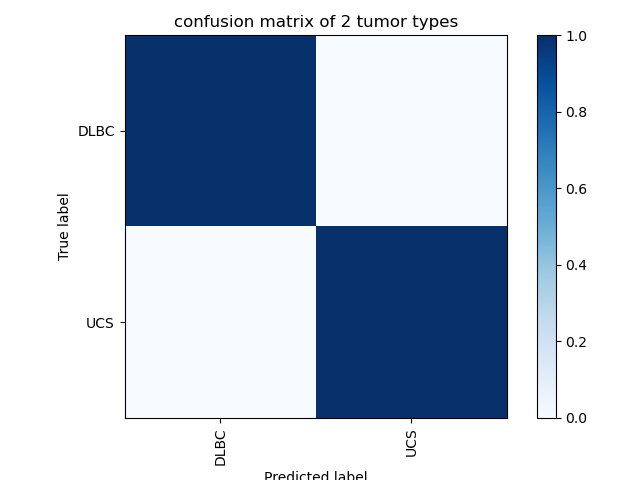
\includegraphics[width=0.7\textwidth]{images/cnfMatrices/cnf_matrix_caso_binario.png}
    \caption{La matrice di confusione del caso binario}
    \label{fig:cnf_matrix_binary}
\end{figure}

% 4.1.2
\subsubsection{Caso Ternario}
Come per il caso binario, anche per il caso ternario è stato necessario modificare la soglia di varianza utilizzata
nella fase di preprocessing per l'estrazione delle feature (i geni). La soglia utilizzata in questo caso è stata di
$0.9869$ e ci ha permesso di avere $10382$ geni. Le performance ottenute in questo test sono riportate in Tabella
\ref{tab:ternary_score} a pagina \pageref{tab:ternary_score} mentre l'accuracy divisa
per coorte tumorale è riportata in Tabella \ref{tab:tern_test_res} a pagina \pageref{tab:tern_test_res}. 
Per completezza, abbiamo generato anche la matrice di confusione riportata in Figura \ref{fig:cnf_matrix_ternary} 
dalla quale si evince che BLCA è stata identificata al 97.56\% correttamente e solo nel 2.44\% è stata 
identificata come CESC; CESC è stata sempre identificata correttamente; LGG è stata identificata correttamente al
98.04\% mentre è stata identificata all'1.96\% come BLCA. 

% Tabella: [Caso Ternario] Performance
\begin{table}[h!]
    \centering
    \caption{Performance del caso ternario}
    \begin{tabular}{crrrr}
        \toprule
         Metodo & Accuracy & Precision & Recall & F1-score \\
         \midrule
         CNN    & 98.37\%    & 98.45\%     & 98.37\%  & 98.37\%     \\
         \bottomrule
    \end{tabular}
    \label{tab:ternary_score}
\end{table}
% Tabella: [Caso Ternario] Accuracy per coorte tumorale
\begin{table}[htbp!]
    \centering 
    \caption{Risultati del caso ternario per coorte tumorale}
    %\large{
    \begin{tabular}{llrrrr}
    \toprule
    Classe   & Coorte & Numero   & Accuratezza & Accuratezza & Accuratezza \\
    tumorale &        & Campioni & ns. metodo  & Variante    & Riferimento \\
    \midrule
    Bladder urothelial carcinoma                    & BLCA & $408$  & 0.98 & & 0.97 \\
    Cervical and endocervical cancers               & CESC & $304$  & 1.00 & & 0.93 \\
    Brain Lower Grade Glioma                        & LGG  & $516$  & 0.98 & & 0.98 \\  
    \midrule
    \textbf{Totale campioni}                        &      & $\mathbf{1.228}$  \\
    \bottomrule
    \label{tab:tern_test_res}
    \end{tabular} 
    %}
\end{table}
% Figura: [Caso Ternario] Matrice di Confusione
\begin{figure}
    \centering
    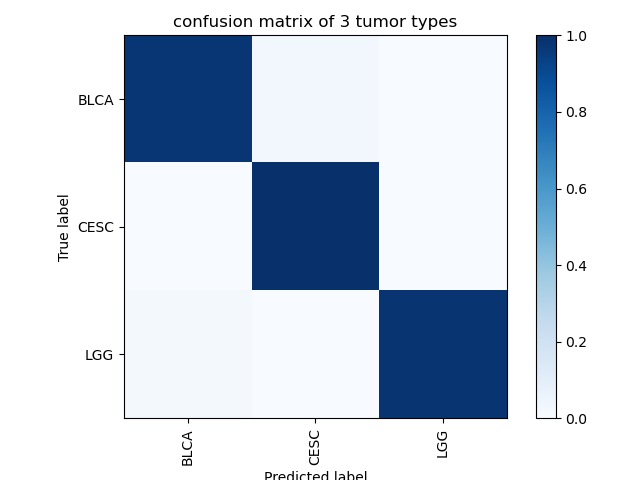
\includegraphics[width=0.7\textwidth]{images/cnfMatrices/cnf_matrix_caso_ternario.png}
    \caption{La matrice di confusione del caso ternario}
    \label{fig:cnf_matrix_ternary}
\end{figure}

% 4.1.3
\subsubsection{Caso Generale}
Le performance ottenute nel test generale usando la rete neurale di \cite{lyu2018deep} sono riportati nella 
Tabella \ref{tab:method_score} a pagina \pageref{tab:method_score} mentre una comparazione dell'accuracy per ogni
classe tumorale è mostrata in Tabella \ref{tab:GPU-res} a pagina \pageref{tab:GPU-res}.
Inoltre, abbiamo anche generato la matrice di confusione così come mostrato in Figura \ref{fig:cnf_matrix_general}.
Dalla matrice di confusione si può notare che la maggior parte delle classi sono classificate correttamente, 
tuttavia ci sono alcune classificazioni errate: 
\begin{enumerate}
    \item i campioni READ sono per lo più sono classificati come COAD e ciò potrebbe essere dovuto alla
          vicinanza delle locazioni spaziali dei due tumori; 
    \item alcuni campioni di CHOL sono classificati erroneamente come LIHC a causa dei pochi campioni presenti per 
          la classe CHOL;
    \item alcuni campioni di ESCA sono classificati erroneamente come STAD;
    \item alcuni campioni di UCS sono classificati erroneamente come UCEC.
\end{enumerate}
Delle possibili motivazioni per gli errori di classificazione (3) e (4) sono riportate nel paragrafo 
\ref{subsec:class-val-varnet} in quanto si sono riscontrate anche durante l'utilizzo della rete VarNet.
% Tabella: [Caso Generale] Performance
\begin{table}[htbp!]
    \centering
    \caption{Performance del metodo utilizzato}
    \begin{tabular}{crrrr}
        \toprule
         Metodo & Accuracy & Precision & Recall & F1-score \\
         \midrule
         CNN    & 95.79\%    & 95.95\%     & 95.79\%  & 95.57\%     \\
         \bottomrule
    \end{tabular}
    \label{tab:method_score}
\end{table}

% Tabella - [VarNet] Accuracy per coorte tumorale
\begin{table}[h!]
    \centering 
    \caption{Accuracy per coorte tumorale (calcolo effettuato su GPU e su dataset con oversampling).}
    \large{
    \begin{tabular}{lrrr}
    \toprule
     Coorte  & Accuratezza & Accuratezza & Accuratezza \\
             & ns. metodo  & Variante    & Riferimento \\
    \midrule
     ACC  & \textbf{1.00} & \textbf{1.00} & 0.95 \\
     BLCA &  \textbf{0.98} & \textbf{0.98} & 0.97 \\
     BRCA &  \textbf{1.00} &\textbf{ 1.00} & 0.99 \\
     CESC &  \textbf{0.97} & \textbf{0.97} & 0.93 \\
     CHOL &  \textbf{0.60} & \textbf{0.60} & 0.56 \\
     COAD &  \textbf{1.00} & \textbf{0.97} & 0.95 \\
     DLBC &  1.00 & 1.00 & 1.00 \\
     ESCA &  \textcolor{blue}{0.75} & \textbf{0.85} & 0.77 \\
     GBM  &  \textbf{1.00} & \textbf{1.00} & 0.94 \\
     HNSC &  0.98 & \textbf{1.00} & 0.98 \\
     KICH &  \textcolor{blue}{0.67} & \textcolor{blue}{0.44} & 0.87 \\
     KIRC &  \textcolor{blue}{0.87} & \textcolor{blue}{0.87} & 0.95 \\
     KIRP &  \textbf{0.94} & \textbf{0.94} & 0.93 \\
     LAML &  1.00 & 1.00 & 1.00 \\
     LGG  &  0.98 & \textbf{1.00} & 0.98 \\
     LIHC &  \textbf{1.00} & \textbf{1.00} & 0.97 \\
     LUAD &  \textcolor{blue}{0.91} & \textbf{0.97} & 0.95 \\
     LUSC &  \textcolor{blue}{0.89} & \textcolor{blue}{0.89} & 0.91 \\
     MESO &  \textbf{1.00} & \textcolor{blue}{0.89} & 0.94 \\
     OV   &  \textcolor{blue}{0.97} & \textbf{1.00} & 0.99 \\
     PAAD &  \textcolor{blue}{0.95} & \textcolor{blue}{0.95} & 0.97 \\
     PCPG &  1.00 & 1.00 & 1.00 \\
     PRAD &  1.00 & 1.00 & 1.00 \\
     READ &  \textcolor{blue}{\textbf{0.09}} & \textcolor{blue}{\textbf{0.09}} & 0.35 \\ 
     SARC &  \textcolor{blue}{0.92} & \textcolor{blue}{0.85} & 0.97 \\ 
     SKCM &  \textcolor{blue}{0.96} & \textcolor{blue}{0.96} & 0.98 \\ 
     STAD &  \textcolor{blue}{0.93} & \textbf{0.98} & 0.96 \\ 
     TGCT &  \textbf{1.00} & \textbf{1.00} & 0.99 \\ 
     THCA &  1.00 & 1.00 & 1.00 \\ 
     THYM &  \textbf{1.00} & \textcolor{blue}{0.92} & 0.99 \\ 
     UCEC &  \textbf{1.00} & \textcolor{blue}{0.95} & 0.96 \\ 
     UCS  &  \textbf{0.83} & \textcolor{blue}{0.67} & 0.81 \\ 
     UVM  &  \textbf{1.00} & \textbf{1.00} & 0.99 \\ 
    \bottomrule
    \label{tab:GPU-res}
    \end{tabular} 
    } %end large
\end{table}
Dal momento che il nostro metodo, al pari di \cite{lyu2018deep} si prefissava di classificare i tumori
e allo stesso tempo individuare i potenziali biomarker, sono stati mantenuti molti geni nella fase
di preprocessing.

% Figura: [Caso Generale] Matrice di Confusione
\begin{figure}[htbp!]
    \centering
    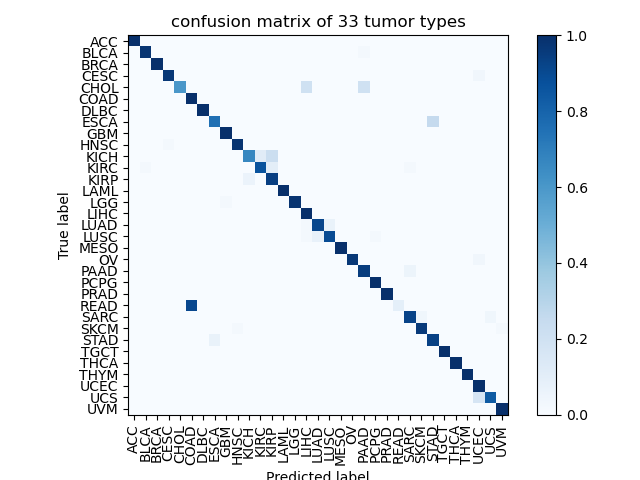
\includegraphics[width=0.7\textwidth]{images/cnfMatrices/cnf_matrix.png}
    \caption{La matrice di confusione del caso generale}
    \label{fig:cnf_matrix_general}
\end{figure}

% 4.2
\subsection{Heat-Map Generate}
\label{subsec:gen_heatmap}
Nelle seguenti sottosezioni saranno mostrati degli esempi di heatmap generate per i vari casi di test effettuati.
Le zone indicate da un contorno \textcolor{red}{rosso} nelle immagini indicano le zone con i pixel più luminosi, ossia
i geni che hanno contribuito maggiormente alla classificazione.

% 4.2.1
\subsubsection{Caso Binario}
Alcuni esempi di heatmap generate nel caso binario sono mostrate nella Figura \ref{fig:bin-heatmap} a pagina 
\pageref{fig:bin-heatmap}.
Si può notare che esiste una certa similarità nelle immagini e in particolare, per DLBC, è possibile
notare lo stesso pattern per le fold 2, 3, 4 e 9.

	\begin{figure}[htpb!]
		\centering
		% prima riga
		\subfloat[][]{
\includegraphics[scale=0.15]{images/bin-heatmaps/DLBCTitle}} \hfill
		\subfloat[][]{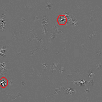
\includegraphics[scale=0.7]{images/bin-heatmaps/DLBCFold0}} \hfill % 1
		\subfloat[][]{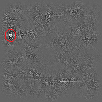
\includegraphics[scale=0.7]{images/bin-heatmaps/DLBCFold1}} \hfill % 2
		\subfloat[][]{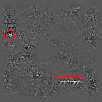
\includegraphics[scale=0.7]{images/bin-heatmaps/DLBCFold2}} \hfill % 3
		\subfloat[][]{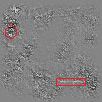
\includegraphics[scale=0.7]{images/bin-heatmaps/DLBCFold3}} \hfill % 4
		\subfloat[][]{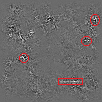
\includegraphics[scale=0.7]{images/bin-heatmaps/DLBCFold4}} \hfill % 5
		\subfloat[][]{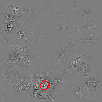
\includegraphics[scale=0.7]{images/bin-heatmaps/DLBCFold5}} \hfill % 6
		\subfloat[][]{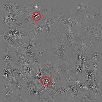
\includegraphics[scale=0.7]{images/bin-heatmaps/DLBCFold6}} \hfill % 7
		\subfloat[][]{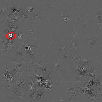
\includegraphics[scale=0.7]{images/bin-heatmaps/DLBCFold7}} \hfill % 8
		\subfloat[][]{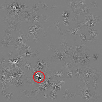
\includegraphics[scale=0.7]{images/bin-heatmaps/DLBCFold8}} \hfill % 9
		\subfloat[][]{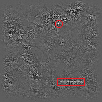
\includegraphics[scale=0.7]{images/bin-heatmaps/DLBCFold9}} \\     % 10
	   \vspace{-5mm}
		% seconda riga
		\subfloat[][]{
\includegraphics[scale=0.15]{images/bin-heatmaps/UCSTitle}} \hfill
		\subfloat[][]{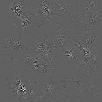
\includegraphics[scale=0.7]{images/bin-heatmaps/UCSFold0}} \hfill % 11
		\subfloat[][]{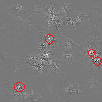
\includegraphics[scale=0.7]{images/bin-heatmaps/UCSFold1}} \hfill % 12
		\subfloat[][]{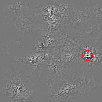
\includegraphics[scale=0.7]{images/bin-heatmaps/UCSFold2}} \hfill % 13
		\subfloat[][]{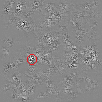
\includegraphics[scale=0.7]{images/bin-heatmaps/UCSFold3}} \hfill % 14
		\subfloat[][]{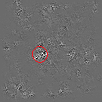
\includegraphics[scale=0.7]{images/bin-heatmaps/UCSFold4}} \hfill % 15
		\subfloat[][]{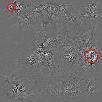
\includegraphics[scale=0.7]{images/bin-heatmaps/UCSFold5}} \hfill % 16
		\subfloat[][]{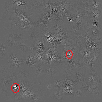
\includegraphics[scale=0.7]{images/bin-heatmaps/UCSFold6}} \hfill % 17
		\subfloat[][]{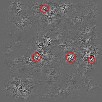
\includegraphics[scale=0.7]{images/bin-heatmaps/UCSFold7}} \hfill % 18
		\subfloat[][]{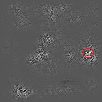
\includegraphics[scale=0.7]{images/bin-heatmaps/UCSFold8}} \hfill % 19
		\subfloat[][]{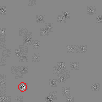
\includegraphics[scale=0.7]{images/bin-heatmaps/UCSFold9}} \\     % 20
		\caption{Heatmaps del caso binario}
		\label{fig:bin-heatmap}
	\end{figure}

% 4.2.2
\subsubsection{Caso Ternario}
Alcuni esempi di heatmap generate nel caso ternario sono mostrate nella Figura \ref{fig:tern-heatmap} a
pagina \pageref{fig:tern-heatmap}.
Anche in questo caso si può notare che esiste una certa similarità nelle immagini ma purtroppo
non è presente nessun pattern evidente.

	\begin{figure}[htpb!]
		\centering
		% prima riga
		\subfloat[][]{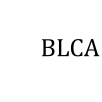
\includegraphics[scale=0.15]{images/tern-heatmaps/BLCATitle}} \hfill
		\subfloat[][]{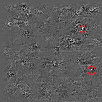
\includegraphics[scale=0.7]{images/tern-heatmaps/BLCAFold0}} \hfill % 1
		\subfloat[][]{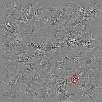
\includegraphics[scale=0.7]{images/tern-heatmaps/BLCAFold1}} \hfill % 2
		\subfloat[][]{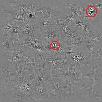
\includegraphics[scale=0.7]{images/tern-heatmaps/BLCAFold2}} \hfill % 3
		\subfloat[][]{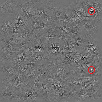
\includegraphics[scale=0.7]{images/tern-heatmaps/BLCAFold3}} \hfill % 4
		\subfloat[][]{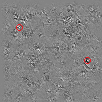
\includegraphics[scale=0.7]{images/tern-heatmaps/BLCAFold4}} \hfill % 5
		\subfloat[][]{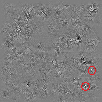
\includegraphics[scale=0.7]{images/tern-heatmaps/BLCAFold5}} \hfill % 6
		\subfloat[][]{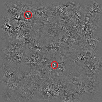
\includegraphics[scale=0.7]{images/tern-heatmaps/BLCAFold6}} \hfill % 7
		\subfloat[][]{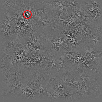
\includegraphics[scale=0.7]{images/tern-heatmaps/BLCAFold7}} \hfill % 8
		\subfloat[][]{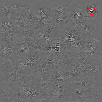
\includegraphics[scale=0.7]{images/tern-heatmaps/BLCAFold8}} \hfill % 9
		\subfloat[][]{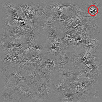
\includegraphics[scale=0.7]{images/tern-heatmaps/BLCAFold9}} \\     % 10
	   \vspace{-5mm}
		% seconda riga
		\subfloat[][]{
\includegraphics[scale=0.15]{images/tern-heatmaps/CESCTitle}} \hfill
		\subfloat[][]{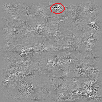
\includegraphics[scale=0.7]{images/tern-heatmaps/CESCFold0}} \hfill % 11
		\subfloat[][]{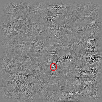
\includegraphics[scale=0.7]{images/tern-heatmaps/CESCFold1}} \hfill % 12
		\subfloat[][]{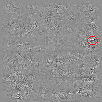
\includegraphics[scale=0.7]{images/tern-heatmaps/CESCFold2}} \hfill % 13
		\subfloat[][]{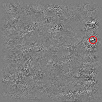
\includegraphics[scale=0.7]{images/tern-heatmaps/CESCFold3}} \hfill % 14
		\subfloat[][]{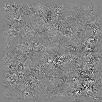
\includegraphics[scale=0.7]{images/tern-heatmaps/CESCFold4}} \hfill % 15
		\subfloat[][]{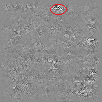
\includegraphics[scale=0.7]{images/tern-heatmaps/CESCFold5}} \hfill % 16
		\subfloat[][]{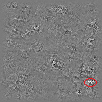
\includegraphics[scale=0.7]{images/tern-heatmaps/CESCFold6}} \hfill % 17
		\subfloat[][]{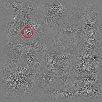
\includegraphics[scale=0.7]{images/tern-heatmaps/CESCFold7}} \hfill % 18
		\subfloat[][]{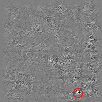
\includegraphics[scale=0.7]{images/tern-heatmaps/CESCFold8}} \hfill % 19
		\subfloat[][]{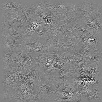
\includegraphics[scale=0.7]{images/tern-heatmaps/CESCFold9}} \\     % 20
		\vspace{-5mm}
			% terza riga
		\subfloat[][]{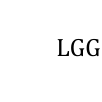
\includegraphics[scale=0.15]{images/tern-heatmaps/LGGTitle}} \hfill
		\subfloat[][]{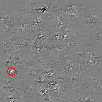
\includegraphics[scale=0.7]{images/tern-heatmaps/LGGFold0}} \hfill % 21
		\subfloat[][]{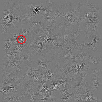
\includegraphics[scale=0.7]{images/tern-heatmaps/LGGFold1}} \hfill % 22
		\subfloat[][]{\includegraphics[scale=0.7]{images/tern-heatmaps/LGGFold2}} \hfill % 23
		\subfloat[][]{\includegraphics[scale=0.7]{images/tern-heatmaps/LGGFold3}} \hfill % 24
		\subfloat[][]{\includegraphics[scale=0.7]{images/tern-heatmaps/LGGFold4}} \hfill % 25
		\subfloat[][]{\includegraphics[scale=0.7]{images/tern-heatmaps/LGGFold5}} \hfill % 26
		\subfloat[][]{\includegraphics[scale=0.7]{images/tern-heatmaps/LGGFold6}} \hfill % 27
		\subfloat[][]{\includegraphics[scale=0.7]{images/tern-heatmaps/LGGFold7}} \hfill % 28
		\subfloat[][]{\includegraphics[scale=0.7]{images/tern-heatmaps/LGGFold8}} \hfill % 29
		\subfloat[][]{\includegraphics[scale=0.7]{images/tern-heatmaps/LGGFold9}} \\     % 30
		\caption{Heatmaps del caso ternario}
		\label{fig:tern-heatmap}
	\end{figure}

% 4.2.3
\subsubsection{Caso Generale}
Le heatmap generate per ogni classe mostrano una similarità tra le 10 fold e mostrano un pattern distinto
quando comparate tra classi. Alcuni esempi sono mostrati nella Figura \ref{fig:esempi-heatmap} a
pagina \pageref{fig:esempi-heatmap}. 
Nell'esempio, ogni riga rappresenta le heatmap di diverse fold (da sinistra a destra sono dalla fold 1 alla fold 10).
Anche se ci sono alcune differenze tra le diverse fold, esiste un pattern chiaro tra di esse.
\begin{figure}[htpb!]
    \centering
    % prima riga
    \subfloat[][]{\includegraphics[scale=0.3]{images/coloredHeatmapsNet/BLCAtitle}} \hfill
    \subfloat[][]{\includegraphics[scale=0.3]{images/coloredHeatmapsNet/BLCAAvgGuidedGcamNormFold0marked}} \hfill % 1
    \subfloat[][]{\includegraphics[scale=0.3]{images/coloredHeatmapsNet/BLCAAvgGuidedGcamNormFold1marked}} \hfill % 2
    \subfloat[][]{\includegraphics[scale=0.3]{images/coloredHeatmapsNet/BLCAAvgGuidedGcamNormFold2marked}} \hfill % 3
    \subfloat[][]{\includegraphics[scale=0.3]{images/coloredHeatmapsNet/BLCAAvgGuidedGcamNormFold3marked}} \hfill % 4
    \subfloat[][]{\includegraphics[scale=0.3]{images/coloredHeatmapsNet/BLCAAvgGuidedGcamNormFold4marked}} \hfill % 5
    \subfloat[][]{\includegraphics[scale=0.3]{images/coloredHeatmapsNet/BLCAAvgGuidedGcamNormFold5marked}} \hfill % 6
    \subfloat[][]{\includegraphics[scale=0.3]{images/coloredHeatmapsNet/BLCAAvgGuidedGcamNormFold6marked}} \hfill % 7
    \subfloat[][]{\includegraphics[scale=0.3]{images/coloredHeatmapsNet/BLCAAvgGuidedGcamNormFold7marked}} \hfill % 8
    \subfloat[][]{\includegraphics[scale=0.3]{images/coloredHeatmapsNet/BLCAAvgGuidedGcamNormFold8marked}} \hfill % 9
    \subfloat[][]{\includegraphics[scale=0.3]{images/coloredHeatmapsNet/BLCAAvgGuidedGcamNormFold9marked}} \\     % 10
   \vspace{-5mm}
    % seconda riga
    \subfloat[][]{\includegraphics[scale=0.3]{images/coloredHeatmapsNet/LGGtitle}} \hfill
    \subfloat[][]{\includegraphics[scale=0.3]{images/coloredHeatmapsNet/LGGAvgGuidedGcamNormFold0marked}} \hfill % 11
    \subfloat[][]{\includegraphics[scale=0.3]{images/coloredHeatmapsNet/LGGAvgGuidedGcamNormFold1marked}} \hfill % 12
    \subfloat[][]{\includegraphics[scale=0.3]{images/coloredHeatmapsNet/LGGAvgGuidedGcamNormFold2marked}} \hfill % 13
    \subfloat[][]{\includegraphics[scale=0.3]{images/coloredHeatmapsNet/LGGAvgGuidedGcamNormFold3marked}} \hfill % 14
    \subfloat[][]{\includegraphics[scale=0.3]{images/coloredHeatmapsNet/LGGAvgGuidedGcamNormFold4marked}} \hfill % 15
    \subfloat[][]{\includegraphics[scale=0.3]{images/coloredHeatmapsNet/LGGAvgGuidedGcamNormFold5marked}} \hfill % 16
    \subfloat[][]{\includegraphics[scale=0.3]{images/coloredHeatmapsNet/LGGAvgGuidedGcamNormFold6marked}} \hfill % 17
    \subfloat[][]{\includegraphics[scale=0.3]{images/coloredHeatmapsNet/LGGAvgGuidedGcamNormFold7marked}} \hfill % 18
    \subfloat[][]{\includegraphics[scale=0.3]{images/coloredHeatmapsNet/LGGAvgGuidedGcamNormFold8marked}} \hfill % 19
    \subfloat[][]{\includegraphics[scale=0.3]{images/coloredHeatmapsNet/LGGAvgGuidedGcamNormFold9marked}} \\     % 20
    \vspace{-5mm}
    % terza riga
    \subfloat[][]{\includegraphics[scale=0.3]{images/coloredHeatmapsNet/PRADtitle}} \hfill
    \subfloat[][]{\includegraphics[scale=0.3]{images/coloredHeatmapsNet/PRADAvgGuidedGcamNormFold0marked}} \hfill % 21
    \subfloat[][]{\includegraphics[scale=0.3]{images/coloredHeatmapsNet/PRADAvgGuidedGcamNormFold1marked}} \hfill % 22
    \subfloat[][]{\includegraphics[scale=0.3]{images/coloredHeatmapsNet/PRADAvgGuidedGcamNormFold2marked}} \hfill % 23
    \subfloat[][]{\includegraphics[scale=0.3]{images/coloredHeatmapsNet/PRADAvgGuidedGcamNormFold3marked}} \hfill % 24
    \subfloat[][]{\includegraphics[scale=0.3]{images/coloredHeatmapsNet/PRADAvgGuidedGcamNormFold4marked}} \hfill % 25
    \subfloat[][]{\includegraphics[scale=0.3]{images/coloredHeatmapsNet/PRADAvgGuidedGcamNormFold5marked}} \hfill % 26
    \subfloat[][]{\includegraphics[scale=0.3]{images/coloredHeatmapsNet/PRADAvgGuidedGcamNormFold6marked}} \hfill % 27
    \subfloat[][]{\includegraphics[scale=0.3]{images/coloredHeatmapsNet/PRADAvgGuidedGcamNormFold7marked}} \hfill % 28
    \subfloat[][]{\includegraphics[scale=0.3]{images/coloredHeatmapsNet/PRADAvgGuidedGcamNormFold8marked}} \hfill % 29
    \subfloat[][]{\includegraphics[scale=0.3]{images/coloredHeatmapsNet/PRADAvgGuidedGcamNormFold9marked}} \hfill % 30
    \caption{Alcuni esempi di heatmap. Ogni colonna rappresenta il risultato di una fold. Nella prima riga ci sono le heatmap %
                del tipo di tumore BLCA, nella seconda di LGG e nella terza di PRAD.}
    \label{fig:esempi-heatmap}
\end{figure}

% 4.3
\subsection{Validazione dei percorsi biologici dei top genes}
\label{ssec:val-bio-net}
Come si può notare dalla Figura \ref{fig:confidence-score-Net} a pagina \pageref{fig:confidence-score-Net}, 
l'intensità dei primi 100 geni decresce rapidamente, mentre l'intensità dei geni successivi decresce in maniera 
uniforme. Tale comportamento è stato constatato anche in \cite{lyu2018deep}. Inoltre, quando
l'intensità è bassa, il tasso di decrescita cresce di nuovo. Se, come hanno fatto in \cite{lyu2018deep}, si assume 
che un'intensità più alta implica una \textit{significance} più alta, dal momento che la curva delle intensità nei
primi 400 geni cambia in maniera più evidente (ossia è più grande) rispetto alle altra migliaia di geni, allora 
è lecito scegliere i primi 400 geni come query per effettuare la pathway analysis. In aggiunta, facendo una
comparazione con il numero totale di geni considerati (10381), la scelta di 400 geni è 
consistente col fatto che il numero di biomarker dovrebbe essere basso. Per effettuare la KEGG\footnote{Kyoto
Encyclopedia of Genes and Genomes} pathway analysis è stato utilizzato il tool
DAVID\footnote{\url{https://david.ncifcrf.gov/home.jsp}}.
In seguito, basandoci sui risultati già ottenuti da \cite{lyu2018deep} e facendo una sommaria attività di 
literature review, limitata alla nostra conoscenza attuale, abbiamo provato a trovare le relazioni che sussistono 
tra le pathway individuate e i tipi di tumore. Le pathway individuate, con un P-value inferiore a $10^{-3}$, per 
i casi di test effettuati, sono mostrate nelle successive sezioni.
% Figura - Confidence score
\begin{figure}
    \centering
    \includegraphics[width=0.7\textwidth]{images/confidence-score/ConfidenceScore-plot-Net.png}
    \caption{I cambi di intensità nelle heatmap per ogni classe. Si può notare come alcune classi condividano lo stesso pattern nei
    cambi di intensità.}
    \label{fig:confidence-score-Net}
\end{figure}
Nelle Tabelle che seguiranno si utilizzerà la seguente legenda: i valori di questo \textcolor{\clrnew}{colore} 
sono le nuove pathway rilevate dalle nostre analisi con il tool DAVID, i valori con questo 
\colorbox{\clrmatch}{background} indicano le path che trovano riscontro anche nel lavoro di Lyu e Haque
\cite{lyu2018deep} e i valori con questo \colorbox{\clrpath}{\textbf{background}} indicano quelle pathway che 
sono specifiche della coorte tumorale.
\subsubsection{Caso Binario}~\newline
Come si può notare dalla Tabella che segue, le pathway ottenute in questo caso binario, a differenza delle
stesse classi tumorali riportate nella sezione \ref{ssec:val-bio-net}, sono molte di più e, a differenza
di quanto rilevato in \cite{lyu2018deep} nel 2018, sono presenti anche malattie di origini recente (ad es. il Corona
Virus).
Per UCS inoltre, si può notare che sono presenti quattro pathway tumorali note: Wnt signaling pathway, PI3K-Akt
signaling pathway, Hippo signaling pathway e TGF-beta signaling pathway, tre delle quali (Wnt, Hippo e TGF-beta)
scompaiono nel caso generale descritto nella sezione \ref{ssec:val-bio-net}.

Tali risultati sono ottenuti in quanto il numero di classi in esame è molto piccolo e dunque, al momento della
classificazione, non viene sfruttata la conoscenza di ulteriori classi tumorali e in sede di generazione delle heatmap, 
e quindi di attribuzione del significance score ai geni (dal momento che si scopre quali geni hanno contribuito di più 
alla classificazione), il valore che viene assegnato ai geni è diverso e quindi ne consegue che anche la selezione 
dei top 400 effettuata in questo caso è diversa rispetto al caso generale.
\begin{longtable}{cllr}
%intestazione iniziale
\caption{Risultati della Pathways Analysis sui primi 400 geni per le coorti DLBC e UCS ($P < 10^{-3}$)} \\
\toprule
\multirow{2}{*}{Tumore} & \multicolumn{2}{l}{Pathway correlata} & \multirow{2}{*}{P value} \\
& ID & Nome \\
\midrule
\endfirsthead
\toprule
\multirow{2}{*}{Tumore} & \multicolumn{2}{l}{Pathway correlata} & \multirow{2}{*}{P value} \\
& ID & Nome \\
\midrule
\endhead
\midrule
\multicolumn{2}{r}{Continua nella prossima pagina}
\endfoot
\bottomrule
\endlastfoot
DLBC & hsa05169 & \textcolor{\clrnew}{Epstein-Barr virus infection} & 1.43e-16\\ 
 \rowcolor{\clrmatch} & hsa05166 & Human T-cell leukemia virus 1 infection & 1.01e-13 \\ 
 & hsa04659 & \textcolor{\clrnew}{Th17 cell differentiation} & 1.28e-13 \\ 
 & hsa04658 & \textcolor{\clrnew}{Th1 and Th2 cell differentiation} & 3.13e-13 \\ 
 \rowcolor{\clrpath} & hsa04062 & \textbf{Chemokine signaling pathway} & 3.10e-12 \\ 
 \rowcolor{\clrpath} & hsa05330 & \textbf{Allograft rejection} & 9.20e-12 \\ 
 \rowcolor{\clrmatch} & hsa04612 & Antigen processing and presentation & 5.07e-11 \\ 
 \rowcolor{\clrmatch} & hsa05140 & Leishmaniasis & 1.94e-10 \\ 
 \rowcolor{\clrmatch}& hsa04940 & Type I diabetes mellitus & 2.02e-10 \\ 
 \rowcolor{\clrpath} & hsa05332 & \textbf{Graft-versus-host disease} & 9.73e-10 \\ 
 \rowcolor{\clrmatch} & hsa05145 & Toxoplasmosis & 1.02e-09 \\ 
 \rowcolor{\clrmatch} & hsa05416 & Viral myocarditis & 1.72e-09 \\ 
 \rowcolor{\clrpath} & hsa04064 & \textbf{NF-kappa B signaling pathway} & 1.98e-09 \\ 
 \rowcolor{\clrmatch} & hsa05321 & Inflammatory bowel disease & 2.09e-09 \\ 
 & hsa04380 & \textcolor{\clrnew}{Osteoclast differentiation} & 3.82e-09 \\ 
 & hsa04668 & \textcolor{\clrnew}{TNF signaling pathway} & 4.10e-09 \\ 
 & hsa05340 & \textcolor{\clrnew}{Primary immunodeficiency} & 7.56e-09 \\ 
 & hsa04061 & \textcolor{\clrnew}{Viral protein interaction with cytokine and cytokine receptor} & 4.56e-08 \\ 
 & hsa05200 & \textcolor{\clrnew}{Pathways in cancer} & 8.57e-08 \\ 
 \rowcolor{\clrmatch} & hsa05323 & Rheumatoid arthritis & 1.18e-07 \\ 
 & hsa05163 & \textcolor{\clrnew}{Human cytomegalovirus infection} & 1.19e-07 \\ 
 \rowcolor{\clrmatch} & hsa05320 & Autoimmune thyroid disease & 1.26e-07 \\ 
 \rowcolor{\clrmatch} & hsa04672 & Intestinal immune network for IgA production & 1.57e-07 \\ 
 \rowcolor{\clrmatch} & hsa05150 & Staphylococcus aureus infection & 2.47e-07 \\ 
 & hsa05167 & \textcolor{\clrnew}{Kaposi sarcoma-associated herpesvirus infection} & 3.78e-07 \\ 
 \rowcolor{\clrpath} & hsa04514 & \textbf{Cell adhesion molecules} & 4.20e-07 \\ 
 \rowcolor{\clrpath} & hsa04662 & \textbf{B cell receptor signaling pathway} & 4.29e-07 \\ 
 \rowcolor{\clrmatch} & hsa04060 & Cytokine-cytokine receptor interaction & 4.36e-07 \\ 
 & hsa05417 & \textcolor{\clrnew}{Lipid and atherosclerosis} & 4.78e-07 \\ 
 \rowcolor{\clrmatch} & hsa04640 & Hematopoietic cell lineage & 4.99e-07 \\ 
 \rowcolor{\clrmatch} & hsa05310 & Asthma & 7.56e-07 \\ 
 \rowcolor{\clrmatch} & hsa05152 & Tuberculosis & 8.38e-07 \\ 
 \rowcolor{\clrmatch} & hsa04145 & Phagosome & 1.48e-06 \\ 
 & hsa04933 & \textcolor{\clrnew}{AGE-RAGE signaling pathway in diabetic complications} & 2.16e-06 \\ 
 & hsa05130 & \textcolor{\clrnew}{Pathogenic Escherichia coli infection} & 3.86e-06 \\ 
 & hsa05170 & \textcolor{\clrnew}{Human immunodeficiency virus 1 infection} & 4.80e-06 \\ 
 & hsa04210 & \textcolor{\clrnew}{Apoptosis} & 6.52e-06 \\ 
 & hsa05171 & \textcolor{\clrnew}{Coronavirus disease - COVID-19} & 1.05e-05 \\ 
 & hsa05162 & \textcolor{\clrnew}{Measles} & 1.06e-05 \\ 
 & hsa05205 & \textcolor{\clrnew}{Proteoglycans in cancer} & 1.10e-05 \\ 
 & hsa04611 & \textcolor{\clrnew}{Platelet activation} & 1.98e-05 \\ 
 & hsa05418 & \textcolor{\clrnew}{Fluid shear stress and atherosclerosis} & 2.83e-05 \\ 
 & hsa04670 & \textcolor{\clrnew}{Leukocyte transendothelial migration} & 3.00e-05 \\ 
 & hsa05142 & \textcolor{\clrnew}{Chagas disease} & 3.17e-05 \\ 
 & hsa04926 & \textcolor{\clrnew}{Relaxin signaling pathway} & 4.36e-05 \\ 
 & hsa04015 & \textcolor{\clrnew}{Rap1 signaling pathway} & 4.60e-05 \\ 
 & hsa05164 & \textcolor{\clrnew}{Influenza A} & 6.03e-05 \\ 
 & hsa05215 & \textcolor{\clrnew}{Prostate cancer} & 1.12e-04 \\ 
 & hsa04625 & \textcolor{\clrnew}{C-type lectin receptor signaling pathway} & 1.27e-04 \\ 
 & hsa05202 & \textcolor{\clrnew}{Transcriptional misregulation in cancer} & 1.58e-04 \\ 
 & hsa05161 & \textcolor{\clrnew}{Hepatitis B} & 2.46e-04 \\ 
 & hsa04218 & \textcolor{\clrnew}{Cellular senescence} & 2.74e-04 \\ 
 & hsa04010 & \textcolor{\clrnew}{MAPK signaling pathway} & 2.82e-04 \\ 
 & hsa04620 & \textcolor{\clrnew}{Toll-like receptor signaling pathway} & 3.39e-04 \\ 
 & hsa04660 & \textcolor{\clrnew}{T cell receptor signaling pathway} & 3.39e-04 \\ 
 & hsa04610 & \textcolor{\clrnew}{Complement and coagulation cascades} & 4.06e-04 \\ 
 & hsa04928 & \textcolor{\clrnew}{Parathyroid hormone synthesis, secretion and action} & 4.52e-04 \\ 
 & hsa05132 & \textcolor{\clrnew}{Salmonella infection} & 5.33e-04 \\ 
 & hsa05133 & \textcolor{\clrnew}{Pertussis} & 6.18e-04 \\ 
 & hsa05219 & \textcolor{\clrnew}{Bladder cancer} & 6.71e-04 \\ 
 & hsa04151 & \textcolor{\clrnew}{PI3K-Akt signaling pathway} & 8.15e-04 \\ 
 & hsa05203 & \textcolor{\clrnew}{Viral carcinogenesis} & 9.87e-04 \\ 
\midrule 
\rowcolor{\clrmatch} UCS & hsa04512 & ECM-receptor interaction & 1.14e-13\\ 
 & hsa05165 & \textcolor{\clrnew}{Human papillomavirus infection} & 3.44e-12 \\ 
 \rowcolor{\clrmatch}& hsa04510 & Focal adhesion & 1.42e-11 \\ 
 & hsa05200 & \textcolor{\clrnew}{Pathways in cancer} & 3.14e-10 \\ 
 & hsa05205 & \textcolor{\clrnew}{Proteoglycans in cancer} & 9.14e-09 \\ 
 & hsa04360 & \textcolor{\clrnew}{Axon guidance} & 1.11e-08 \\ 
 & hsa04810 & \textcolor{\clrnew}{Regulation of actin cytoskeleton} & 2.26e-08 \\ 
 & hsa04310 & \textcolor{\clrnew}{Wnt signaling pathway} & 9.72e-08 \\ 
 & hsa04151 & \textcolor{\clrnew}{PI3K-Akt signaling pathway} & 1.24e-07 \\ 
 \rowcolor{\clrmatch}& hsa04974 & Protein digestion and absorption & 1.48e-07 \\ 
 & hsa05412 & \textcolor{\clrnew}{Arrhythmogenic right ventricular cardiomyopathy} & 1.61e-07 \\ 
 & hsa04514 & \textcolor{\clrnew}{Cell adhesion molecules} & 5.23e-06 \\ 
 & hsa04390 & \textcolor{\clrnew}{Hippo signaling pathway} & 1.36e-05 \\ 
 & hsa04520 & \textcolor{\clrnew}{Adherens junction} & 3.02e-05 \\ 
 & hsa04670 & \textcolor{\clrnew}{Leukocyte transendothelial migration} & 4.25e-05 \\ 
 & hsa05224 & \textcolor{\clrnew}{Breast cancer} & 5.20e-05 \\ 
 & hsa05217 & \textcolor{\clrnew}{Basal cell carcinoma} & 6.10e-05 \\ 
 & hsa05222 & \textcolor{\clrnew}{Small cell lung cancer} & 6.35e-05 \\ 
 & hsa04530 & \textcolor{\clrnew}{Tight junction} & 7.02e-05 \\ 
 & hsa05410 & \textcolor{\clrnew}{Hypertrophic cardiomyopathy} & 1.30e-04 \\ 
 & hsa04015 & \textcolor{\clrnew}{Rap1 signaling pathway} & 1.54e-04 \\ 
 & hsa04933 & \textcolor{\clrnew}{AGE-RAGE signaling pathway in diabetic complications} & 2.46e-04 \\ 
 & hsa04350 & \textcolor{\clrnew}{TGF-beta signaling pathway} & 3.00e-04 \\ 
 & hsa05166 & \textcolor{\clrnew}{Human T-cell leukemia virus 1 infection} & 5.11e-04 \\ 
 & hsa04928 & \textcolor{\clrnew}{Parathyroid hormone synthesis, secretion and action} & 5.99e-04 \\ 
 & hsa05225 & \textcolor{\clrnew}{Hepatocellular carcinoma} & 6.83e-04 \\ 
 & hsa04270 & \textcolor{\clrnew}{Vascular smooth muscle contraction} & 7.20e-04 \\ 
 & hsa04934 & \textcolor{\clrnew}{Cushing syndrome} & 7.56e-04 \\ 
 & hsa05414 & \textcolor{\clrnew}{Dilated cardiomyopathy} & 9.12e-04 \\ 
\midrule 
\end{longtable} 

\subsubsection{Caso Ternario}~\newline
Anche per il caso ternario, così come accaduto per il binario, se si fa un confronto con quanto riportato nella sezione
\ref{ssec:val-bio-net}, è possibile notare che il numero di pathway rilevate per le stesse classi tumorali è maggiore.
Come già indicato nel caso binario, tali risultati sono dovuti al fatto che sono prese in esame poche classi tumorali
e quindi i significance score dei geni sono diversi rispetto al caso generale.
Non è presente un grande differenza con i risultati del caso generale, per cui vale quanto detto nella 
sezione \ref{ssec:val-bio-net} per le stesse classi tumorali.

\begin{longtable}{cllr}
%intestazione iniziale
\caption{Risultati della Pathways Analysis sui primi 400 geni per le coorti BLCA, CESC e LGG ($P < 10^{-3}$)} \\
\toprule
\multirow{2}{*}{Tumore} & \multicolumn{2}{l}{Pathway correlata} & \multirow{2}{*}{P value} \\
& ID & Nome \\
\midrule
\endfirsthead
\toprule
\multirow{2}{*}{Tumore} & \multicolumn{2}{l}{Pathway correlata} & \multirow{2}{*}{P value} \\
& ID & Nome \\
\midrule
\endhead
\midrule
\multicolumn{2}{r}{Continua nella prossima pagina}
\endfoot
\bottomrule
\endlastfoot
\rowcolor{\clrmatch} BLCA & hsa04512 & ECM-receptor interaction & 4.05e-09\\ 
\rowcolor{\clrmatch}& hsa04510 & Focal adhesion & 8.89e-09 \\ 
 & hsa05205 & \textcolor{\clrnew}{Proteoglycans in cancer} & 1.37e-07 \\ 
 & hsa05204 & \textcolor{\clrnew}{Chemical carcinogenesis - DNA adducts} & 5.87e-07 \\ 
 & hsa04514 & \textcolor{\clrnew}{Cell adhesion molecules} & 6.51e-07 \\ 
 \rowcolor{\clrmatch} & hsa00980 & Metabolism of xenobiotics by cytochrome P450 & 5.81e-06 \\ 
 & hsa04145 & \textcolor{\clrnew}{Phagosome} & 1.69e-05 \\ 
 & hsa00983 & \textcolor{\clrnew}{Drug metabolism - other enzymes} & 3.14e-05 \\ 
 & hsa00982 & \textcolor{\clrnew}{Drug metabolism - cytochrome P450} & 6.86e-05 \\ 
 \rowcolor{\clrpath} & hsa00140 & \textbf{Steroid hormone biosynthesis} & 9.77e-05 \\ 
 & hsa05200 & \textcolor{\clrnew}{Pathways in cancer} & 4.02e-04 \\ 
 & hsa04926 & \textcolor{\clrnew}{Relaxin signaling pathway} & 4.53e-04 \\ 
 & hsa00040 & \textcolor{\clrnew}{Pentose and glucuronate interconversions} & 4.62e-04 \\ 
 & hsa05165 & \textcolor{\clrnew}{Human papillomavirus infection} & 4.64e-04 \\ 
 & hsa04360 & \textcolor{\clrnew}{Axon guidance} & 6.36e-04 \\ 
 & hsa04933 & \textcolor{\clrnew}{AGE-RAGE signaling pathway in diabetic complications} & 8.93e-04 \\ 
\midrule 
CESC & hsa04514 & \textcolor{\clrnew}{Cell adhesion molecules} & 6.07e-10\\ 
 & hsa04512 & \textcolor{\clrnew}{ECM-receptor interaction} & 1.37e-07 \\ 
 & hsa05169 & \textcolor{\clrnew}{Epstein-Barr virus infection} & 1.98e-07 \\ 
 & hsa04612 & \textcolor{\clrnew}{Antigen processing and presentation} & 7.53e-07 \\ 
 & hsa04530 & \textcolor{\clrnew}{Tight junction} & 4.43e-06 \\ 
 & hsa05200 & \textcolor{\clrnew}{Pathways in cancer} & 6.27e-06 \\ 
 & hsa05330 & \textcolor{\clrnew}{Allograft rejection} & 6.41e-06 \\ 
 & hsa04940 & \textcolor{\clrnew}{Type I diabetes mellitus} & 6.57e-06 \\ 
 & hsa05166 & \textcolor{\clrnew}{Human T-cell leukemia virus 1 infection} & 7.30e-06 \\ 
 & hsa04510 & \textcolor{\clrnew}{Focal adhesion} & 7.73e-06 \\ 
 & hsa05416 & \textcolor{\clrnew}{Viral myocarditis} & 9.17e-06 \\ 
 & hsa05150 & \textcolor{\clrnew}{Staphylococcus aureus infection} & 1.07e-05 \\ 
 & hsa05332 & \textcolor{\clrnew}{Graft-versus-host disease} & 2.42e-05 \\ 
 & hsa05146 & \textcolor{\clrnew}{Amoebiasis} & 3.19e-05 \\ 
 & hsa05145 & \textcolor{\clrnew}{Toxoplasmosis} & 5.64e-05 \\ 
 \rowcolor{\clrpath}& hsa05205 & \textbf{Proteoglycans in cancer} & 6.76e-05 \\ 
 & hsa04659 & \textcolor{\clrnew}{Th17 cell differentiation} & 8.51e-05 \\ 
 & hsa04145 & \textcolor{\clrnew}{Phagosome} & 1.22e-04 \\ 
 & hsa04658 & \textcolor{\clrnew}{Th1 and Th2 cell differentiation} & 1.56e-04 \\ 
 & hsa04640 & \textcolor{\clrnew}{Hematopoietic cell lineage} & 1.66e-04 \\ 
 & hsa05323 & \textcolor{\clrnew}{Rheumatoid arthritis} & 1.83e-04 \\ 
 & hsa00330 & \textcolor{\clrnew}{Arginine and proline metabolism} & 2.05e-04 \\ 
 & hsa05133 & \textcolor{\clrnew}{Pertussis} & 2.78e-04 \\ 
 & hsa05140 & \textcolor{\clrnew}{Leishmaniasis} & 3.31e-04 \\ 
 & hsa05418 & \textcolor{\clrnew}{Fluid shear stress and atherosclerosis} & 3.44e-04 \\ 
 & hsa04218 & \textcolor{\clrnew}{Cellular senescence} & 4.56e-04 \\ 
 & hsa04670 & \textcolor{\clrnew}{Leukocyte transendothelial migration} & 5.31e-04 \\ 
 & hsa04657 & \textcolor{\clrnew}{IL-17 signaling pathway} & 5.92e-04 \\ 
 & hsa04810 & \textcolor{\clrnew}{Regulation of actin cytoskeleton} & 6.94e-04 \\ 
\midrule 
\rowcolor{\clrpath}LGG & hsa04010 & \textbf{MAPK signaling pathway **} & 1.26e-08\\ 
 & hsa04724 & \textcolor{\clrnew}{Glutamatergic synapse} & 4.80e-08 \\ 
 & hsa04727 & \textcolor{\clrnew}{GABAergic synapse} & 1.05e-06 \\ 
 & hsa04514 & \textcolor{\clrnew}{Cell adhesion molecules} & 5.96e-06 \\ 
 & hsa04713 & \textcolor{\clrnew}{Circadian entrainment} & 6.16e-06 \\ 
 & hsa04728 & \textcolor{\clrnew}{Dopaminergic synapse} & 1.58e-05 \\ 
 & hsa04360 & \textcolor{\clrnew}{Axon guidance} & 3.27e-05 \\ 
 & hsa05200 & \textcolor{\clrnew}{Pathways in cancer} & 1.04e-04 \\ 
 & hsa04725 & \textcolor{\clrnew}{Cholinergic synapse} & 1.08e-04 \\ 
 & hsa05032 & \textcolor{\clrnew}{Morphine addiction} & 1.69e-04 \\ 
 & hsa04015 & \textcolor{\clrnew}{Rap1 signaling pathway} & 3.59e-04 \\ 
 & hsa04014 & \textcolor{\clrnew}{Ras signaling pathway} & 5.50e-04 \\ 
 & hsa04371 & \textcolor{\clrnew}{Apelin signaling pathway} & 6.37e-04 \\ 
 & hsa05031 & \textcolor{\clrnew}{Amphetamine addiction} & 7.16e-04 \\ 
 & hsa05205 & \textcolor{\clrnew}{Proteoglycans in cancer} & 8.80e-04 \\ 
 & hsa04926 & \textcolor{\clrnew}{Relaxin signaling pathway} & 9.72e-04 \\ 
\midrule 
\end{longtable} 

\subsubsection{Caso Generale}~\newline
\label{sssec:bio-val-net}
Come è possibile notare dalla Tabella che segue, a differenza di \cite{lyu2018deep}, sono state trovate pathway per
tutte le classi tumorali ma solo 17 hanno mostrato almeno una pathway collegata allo specifico tipo 
di tumore. I geni contenuti in tali pathway possono essere considerati biomarker specifici del tumore.
Per le classi rimanenti, che non hanno mostrato pathway specifiche correlate alla coorte, sono state
individuate diverse pathway concorrenti. Ad esempio, per le classi ACC, KICH, LGG, PCPG e UVM
è stata rilevata la MAPK signaling pathway che è una nota pathway tumorale che si occupa della sopravvivenza
delle cellule. Analizzando i geni correlati a questa pathway, si può notare che essi non sono gli stessi
per tutte le classi sopramenzionate e dunque tali geni possono essere considerati candidati biomarker.
Stesso discorso può essere fatto per le classi BRCA, CHOL, ESCA, GBM, KIRP, LUSC, PCPG e SARC, che pur non avendo 
mostrato pathway specifiche hanno mostrato la PI3K-Akt signaling che è una nota pathway tumorale per la
sopravvivenza delle cellule proprio come la MAPK signaling pathway. ESCA, GBM e KICH hanno mostrato anche la Hippo
signaling pathway che si occupa di controllare le dimensioni degli organi regolando la proliferazione cellulare, 
l'apoptosi e l'auto-rinnovamento delle cellule staminali e la cui disregolazione è noto contribuisca allo sviluppo 
dei cancri.   
Un'altra considerazione può essere fatta per ESCA, KICH, KIRP, SARC, SKCM, TGCT, THCA e UCS che hanno mostrato
come pathway correlate ECM-receptor e Focal Adhesion e, anche in questo caso, analizzando i geni
correlati a tali pathway, è possibile notare che essi non coincidono per tutte le classi e quindi sono
dei potenziali biomarker.
Una nota a parte meritano la classi CHOL, KICH e READ che, seppur non sono state omesse dai risultati per completezza, 
la loro valenza è relativa in quanto: READ viene ignorata completamente in quanto l'accuracy ottenuta è troppo bassa 
e CHOL e KICH hanno un numero troppo limitato di campioni.
    
\begin{longtable}{cllr}
%intestazione iniziale
\caption{Risultati della Pathways Analysis sui primi 400 geni per ogni tipo di tumore ($P < 10^{-3}$)} \\
\toprule
\multirow{2}{*}{Tumore} & \multicolumn{2}{l}{Pathway correlata} & \multirow{2}{*}{P value} \\
& ID & Nome \\
\midrule
\endfirsthead
\toprule
\multirow{2}{*}{Tumore} & \multicolumn{2}{l}{Pathway correlata} & \multirow{2}{*}{P value} \\
& ID & Nome \\
\midrule
\endhead
\midrule
\multicolumn{2}{r}{Continua nella prossima pagina}
\endfoot
\bottomrule
\endlastfoot
ACC & hsa04010 & \textcolor{\clrnew}{MAPK signaling pathway} & 2.58e-07\\ 
    & hsa04015 & \textcolor{\clrnew}{Rap1 signaling pathway} & 2.65e-05 \\ 
     & hsa04512 & \textcolor{\clrnew}{ECM-receptor interaction} & 3.77e-05 \\ 
     & hsa04976 & \textcolor{\clrnew}{Bile secretion} & 1.33e-04 \\ 
     & hsa04115 & \textcolor{\clrnew}{p53 signaling pathway} & 3.75e-04 \\ 
     & hsa04610 & \textcolor{\clrnew}{Complement and coagulation cascades} & 5.56e-04 \\ 
     & hsa05144 & \textcolor{\clrnew}{Malaria} & 7.06e-04 \\ 
\midrule 
\rowcolor{\clrmatch}BLCA & hsa04512 & ECM-receptor interaction & 9.98e-08\\ 
 & hsa05205 & \textcolor{\clrnew}{Proteoglycans in cancer} & 2.15e-07 \\ 
 & hsa04514 & \textcolor{\clrnew}{Cell adhesion molecules} & 7.48e-06 \\ 
 \rowcolor{\clrmatch}& hsa04510 & Focal adhesion & 1.01e-05 \\ 
 & hsa05150 & \textcolor{\clrnew}{Staphylococcus aureus infection} & 7.54e-05 \\ 
 & hsa04270 & \textcolor{\clrnew}{Vascular smooth muscle contraction} & 1.26e-04 \\ 
 & hsa04668 & \textcolor{\clrnew}{TNF signaling pathway} & 1.64e-04 \\ 
 & hsa05200 & \textcolor{\clrnew}{Pathways in cancer} & 2.11e-04 \\ 
 & hsa04933 & \textcolor{\clrnew}{AGE-RAGE signaling pathway in diabetic complications} & 4.00e-04 \\ 
 & hsa04913 & \textcolor{\clrnew}{Ovarian steroidogenesis} & 5.06e-04 \\ 
 & hsa05165 & \textcolor{\clrnew}{Human papillomavirus infection} & 9.06e-04 \\ 
 & hsa05166 & \textcolor{\clrnew}{Human T-cell leukemia virus 1 infection} & 9.85e-04 \\ 
\midrule 
BRCA & hsa04915 & \textcolor{\clrnew}{Estrogen signaling pathway} & 2.38e-08\\ 
 \rowcolor{\clrmatch}& hsa04512 & ECM-receptor interaction & 2.44e-08 \\ 
 \rowcolor{\clrpath}& hsa04151 & \textbf{PI3K-Akt signaling pathway *} & 4.61e-06 \\ 
 & hsa04927 & \textcolor{\clrnew}{Cortisol synthesis and secretion} & 8.11e-06 \\ 
 & hsa04928 & \textcolor{\clrnew}{Parathyroid hormone synthesis, secretion and action} & 2.10e-05 \\ 
 & hsa04934 & \textcolor{\clrnew}{Cushing syndrome} & 3.31e-05 \\ 
 \rowcolor{\clrmatch}& hsa04510 & Focal adhesion & 4.96e-05 \\ 
 & hsa05205 & \textcolor{\clrnew}{Proteoglycans in cancer} & 8.05e-05 \\ 
 & hsa05165 & \textcolor{\clrnew}{Human papillomavirus infection} & 8.86e-05 \\ 
 \rowcolor{\clrpath}& hsa03320 & \textbf{PPAR signaling pathway *} & 8.95e-05 \\ 
 & hsa04514 & \textcolor{\clrnew}{Cell adhesion molecules} & 1.03e-04 \\ 
 & hsa04145 & \textcolor{\clrnew}{Phagosome} & 1.20e-04 \\ 
 & hsa04933 & \textcolor{\clrnew}{AGE-RAGE signaling pathway in diabetic complications} & 1.51e-04 \\ 
 & hsa05200 & \textcolor{\clrnew}{Pathways in cancer} & 5.14e-04 \\ 
 & hsa01522 & \textcolor{\clrnew}{Endocrine resistance} & 7.22e-04 \\ 
 & hsa04926 & \textcolor{\clrnew}{Relaxin signaling pathway} & 7.76e-04 \\ 
 & hsa04540 & \textcolor{\clrnew}{Gap junction} & 9.62e-04 \\ 
\midrule 
CESC & hsa05200 & \textcolor{\clrnew}{Pathways in cancer} & 8.37e-07\\ 
 & hsa04115 & \textcolor{\clrnew}{p53 signaling pathway} & 4.64e-06 \\ 
 \rowcolor{\clrpath}& hsa05205 & \textbf{Proteoglycans in cancer} & 5.71e-05 \\ 
 & hsa05222 & \textcolor{\clrnew}{Small cell lung cancer} & 8.00e-05 \\ 
 & hsa04512 & \textcolor{\clrnew}{ECM-receptor interaction} & 1.14e-04 \\ 
 & hsa04110 & \textcolor{\clrnew}{Cell cycle} & 1.54e-04 \\ 
 & hsa05146 & \textcolor{\clrnew}{Amoebiasis} & 1.57e-04 \\ 
 & hsa04080 & \textcolor{\clrnew}{Neuroactive ligand-receptor interaction} & 1.79e-04 \\ 
 & hsa04915 & \textcolor{\clrnew}{Estrogen signaling pathway} & 2.85e-04 \\ 
 & hsa04934 & \textcolor{\clrnew}{Cushing syndrome} & 4.46e-04 \\ 
 & hsa05144 & \textcolor{\clrnew}{Malaria} & 5.78e-04 \\ 
\midrule 
CHOL & hsa04512 & \textcolor{\clrnew}{ECM-receptor interaction} & 3.94e-10\\ 
 & hsa04610 & \textcolor{\clrnew}{Complement and coagulation cascades} & 1.92e-08 \\ 
 & hsa00340 & \textcolor{\clrnew}{Histidine metabolism} & 6.82e-06 \\ 
 & hsa04061 & \textcolor{\clrnew}{Viral protein interaction with cytokine and cytokine receptor} & 8.03e-06 \\ 
 & hsa04514 & \textcolor{\clrnew}{Cell adhesion molecules} & 1.59e-05 \\ 
 & hsa04015 & \textcolor{\clrnew}{Rap1 signaling pathway} & 2.18e-05 \\ 
 & hsa04020 & \textcolor{\clrnew}{Calcium signaling pathway} & 3.36e-05 \\ 
 & hsa04510 & \textcolor{\clrnew}{Focal adhesion} & 3.57e-05 \\ 
 & hsa04974 & \textcolor{\clrnew}{Protein digestion and absorption} & 4.25e-05 \\ 
 & hsa04950 & \textcolor{\clrnew}{Maturity onset diabetes of the young} & 4.90e-05 \\ 
 & hsa04540 & \textcolor{\clrnew}{Gap junction} & 6.49e-05 \\ 
 & hsa04080 & \textcolor{\clrnew}{Neuroactive ligand-receptor interaction} & 8.23e-05 \\ 
 & hsa05146 & \textcolor{\clrnew}{Amoebiasis} & 9.96e-05 \\ 
 & hsa04060 & \textcolor{\clrnew}{Cytokine-cytokine receptor interaction} & 1.37e-04 \\ 
 & hsa04928 & \textcolor{\clrnew}{Parathyroid hormone synthesis, secretion and action} & 1.92e-04 \\ 
 & hsa04062 & \textcolor{\clrnew}{Chemokine signaling pathway} & 2.71e-04 \\ 
 & hsa05414 & \textcolor{\clrnew}{Dilated cardiomyopathy} & 6.96e-04 \\ 
 & hsa04530 & \textcolor{\clrnew}{Tight junction} & 8.58e-04 \\ 
 \rowcolor{\clrpath}& hsa04151 & \textbf{PI3K-Akt signaling pathway **} & 8.82e-04 \\ 
\midrule 
COAD & hsa04640 & \textcolor{\clrnew}{Hematopoietic cell lineage} & 6.01e-06\\ 
 & hsa04145 & \textcolor{\clrnew}{Phagosome} & 1.01e-05 \\ 
 & hsa04060 & \textcolor{\clrnew}{Cytokine-cytokine receptor interaction} & 1.18e-05 \\ 
 & hsa04974 & \textcolor{\clrnew}{Protein digestion and absorption} & 1.37e-05 \\ 
 & hsa04512 & \textcolor{\clrnew}{ECM-receptor interaction} & 1.73e-05 \\ 
 & hsa04080 & \textcolor{\clrnew}{Neuroactive ligand-receptor interaction} & 4.12e-05 \\ 
 & hsa04514 & \textcolor{\clrnew}{Cell adhesion molecules} & 5.28e-05 \\ 
 & hsa05332 & \textcolor{\clrnew}{Graft-versus-host disease} & 1.96e-04 \\ 
 & hsa05323 & \textcolor{\clrnew}{Rheumatoid arthritis} & 9.33e-04 \\ 
\midrule 
\rowcolor{\clrmatch}DLBC & hsa04940 & Type I diabetes mellitus & 7.84e-11\\ 
 \rowcolor{\clrpath}& hsa05330 & \textbf{Allograft rejection} & 1.85e-10 \\ 
 \rowcolor{\clrpath}& hsa05332 & \textbf{Graft-versus-host disease} & 3.28e-10 \\ 
 \rowcolor{\clrmatch}& hsa04640 & Hematopoietic cell lineage & 5.58e-10 \\ 
 & hsa04659 & \textcolor{\clrnew}{Th17 cell differentiation} & 6.90e-10 \\ 
 \rowcolor{\clrmatch}& hsa04672 & Intestinal immune network for IgA production & 2.72e-09 \\ 
 \rowcolor{\clrmatch}& hsa04145 & Phagosome & 2.08e-08 \\ 
 \rowcolor{\clrmatch}& hsa05321 & Inflammatory bowel disease & 2.47e-08 \\ 
 \rowcolor{\clrmatch}& hsa05150 & Staphylococcus aureus infection & 4.84e-08 \\ 
 & hsa04658 & \textcolor{\clrnew}{Th1 and Th2 cell differentiation} & 5.35e-08 \\ 
 \rowcolor{\clrmatch}& hsa05323 & Rheumatoid arthritis & 7.22e-08 \\ 
 \rowcolor{\clrmatch}& hsa05416 & Viral myocarditis & 7.58e-08 \\ 
 \rowcolor{\clrmatch}& hsa05140 & Leishmaniasis & 1.01e-07 \\ 
 & hsa04061 & \textcolor{\clrnew}{Viral protein interaction with cytokine and cytokine receptor} & 1.52e-07 \\ 
 \rowcolor{\clrpath}& hsa04514 & \textbf{Cell adhesion molecules} & 1.78e-07 \\ 
 \rowcolor{\clrmatch}& hsa05320 & Autoimmune thyroid disease & 4.97e-07 \\ 
 & hsa04610 & \textcolor{\clrnew}{Complement and coagulation cascades} & 1.50e-06 \\ 
 \rowcolor{\clrpath}& hsa04062 & \textbf{Chemokine signaling pathway} & 2.65e-06 \\ 
 & hsa05169 & \textcolor{\clrnew}{Epstein-Barr virus infection} & 5.57e-06 \\ 
 \rowcolor{\clrmatch}& hsa05166 & Human T-cell leukemia virus 1 infection & 9.70e-06 \\ 
 \rowcolor{\clrmatch}& hsa04060 & Cytokine-cytokine receptor interaction & 1.04e-05 \\ 
 & hsa05133 & \textcolor{\clrnew}{Pertussis} & 1.29e-05 \\ 
 \rowcolor{\clrpath}& hsa04662 & \textbf{B cell receptor signaling pathway} & 1.83e-05 \\ 
 \rowcolor{\clrmatch}& hsa05310 & Asthma & 1.91e-05 \\ 
 & hsa04380 & \textcolor{\clrnew}{Osteoclast differentiation} & 2.74e-05 \\ 
 \rowcolor{\clrmatch}& hsa05152 & Tuberculosis & 1.20e-04 \\ 
 \rowcolor{\clrmatch}& hsa05145 & Toxoplasmosis & 1.51e-04 \\ 
 \rowcolor{\clrmatch}& hsa04612 & Antigen processing and presentation & 1.89e-04 \\ 
 \rowcolor{\clrpath}& hsa04064 & \textbf{NF-kappa B signaling pathway}& 2.26e-04 \\ 
 & hsa04621 & \textcolor{\clrnew}{NOD-like receptor signaling pathway} & 4.09e-04 \\ 
 & hsa05130 & \textcolor{\clrnew}{Pathogenic Escherichia coli infection} & 4.96e-04 \\ 
 & hsa04115 & \textcolor{\clrnew}{p53 signaling pathway} & 5.14e-04 \\ 
 & hsa04625 & \textcolor{\clrnew}{C-type lectin receptor signaling pathway} & 5.46e-04 \\ 
 & hsa04928 & \textcolor{\clrnew}{Parathyroid hormone synthesis, secretion and action} & 7.52e-04 \\ 
\midrule 
\rowcolor{\clrmatch}ESCA & hsa04512 & ECM-receptor interaction & 1.38e-12\\ 
 & hsa05414 & \textcolor{\clrnew}{Dilated cardiomyopathy} & 5.86e-10 \\ 
 \rowcolor{\clrmatch}& hsa05412 & Arrhythmogenic right ventricular cardiomyopathy & 2.79e-09 \\ 
 \rowcolor{\clrmatch}& hsa04510 & Focal adhesion & 2.85e-08 \\ 
 & hsa05410 & \textcolor{\clrnew}{Hypertrophic cardiomyopathy} & 3.42e-08 \\ 
 & hsa05165 & \textcolor{\clrnew}{Human papillomavirus infection} & 2.32e-07 \\ 
 & hsa05200 & \textcolor{\clrnew}{Pathways in cancer} & 2.31e-06 \\ 
 & hsa04022 & \textcolor{\clrnew}{cGMP-PKG signaling pathway} & 1.55e-05 \\ 
 & hsa04151 & \textcolor{\clrnew}{PI3K-Akt signaling pathway *} & 2.25e-05 \\ 
 & hsa05146 & \textcolor{\clrnew}{Amoebiasis} & 6.56e-05 \\ 
 & hsa05222 & \textcolor{\clrnew}{Small cell lung cancer} & 9.19e-05 \\ 
 & hsa04934 & \textcolor{\clrnew}{Cushing syndrome} & 1.02e-04 \\ 
 & hsa05205 & \textcolor{\clrnew}{Proteoglycans in cancer} & 1.50e-04 \\ 
 & hsa04360 & \textcolor{\clrnew}{Axon guidance} & 2.40e-04 \\ 
 & hsa04550 & \textcolor{\clrnew}{Signaling pathways regulating pluripotency of stem cells} & 2.72e-04 \\ 
 & hsa04390 & \textcolor{\clrnew}{Hippo signaling pathway} & 2.99e-04 \\ 
 & hsa04916 & \textcolor{\clrnew}{Melanogenesis} & 4.06e-04 \\ 
 & hsa02010 & \textcolor{\clrnew}{ABC transporters} & 7.09e-04 \\ 
 & hsa05224 & \textcolor{\clrnew}{Breast cancer} & 9.80e-04 \\ 
\midrule 
GBM & hsa04060 & \textcolor{\clrnew}{Cytokine-cytokine receptor interaction} & 4.80e-10\\ 
 & hsa04080 & \textcolor{\clrnew}{Neuroactive ligand-receptor interaction} & 8.72e-10 \\ 
 & hsa04062 & \textcolor{\clrnew}{Chemokine signaling pathway} & 2.85e-06 \\ 
 & hsa04061 & \textcolor{\clrnew}{Viral protein interaction with cytokine and cytokine receptor} & 7.48e-06 \\ 
 & hsa05323 & \textcolor{\clrnew}{Rheumatoid arthritis} & 1.50e-05 \\ 
 & hsa04015 & \textcolor{\clrnew}{Rap1 signaling pathway} & 3.59e-05 \\ 
 & hsa05205 & \textcolor{\clrnew}{Proteoglycans in cancer} & 4.06e-05 \\ 
 & hsa04512 & \textcolor{\clrnew}{ECM-receptor interaction} & 4.60e-05 \\ 
 & hsa04510 & \textcolor{\clrnew}{Focal adhesion} & 5.20e-05 \\ 
 & hsa05144 & \textcolor{\clrnew}{Malaria} & 6.52e-05 \\ 
 & hsa05032 & \textcolor{\clrnew}{Morphine addiction} & 8.44e-05 \\ 
 & hsa05200 & \textcolor{\clrnew}{Pathways in cancer} & 1.93e-04 \\ 
 & hsa04724 & \textcolor{\clrnew}{Glutamatergic synapse} & 2.69e-04 \\ 
 & hsa04020 & \textcolor{\clrnew}{Calcium signaling pathway} & 5.21e-04 \\ 
 & hsa04974 & \textcolor{\clrnew}{Protein digestion and absorption} & 6.78e-04 \\ 
 \rowcolor{\clrpath}& hsa04151 & \textbf{PI3K-Akt signaling pathway **} & 7.09e-04 \\ 
 & hsa04390 & \textcolor{\clrnew}{Hippo signaling pathway} & 7.86e-04 \\ 
 & hsa04371 & \textcolor{\clrnew}{Apelin signaling pathway} & 7.87e-04 \\ 
 & hsa04270 & \textcolor{\clrnew}{Vascular smooth muscle contraction} & 8.89e-04 \\ 
\midrule 
\rowcolor{\clrmatch}HNSC & hsa04512 & ECM-receptor interaction & 5.74e-12\\ 
 \rowcolor{\clrpath}& hsa05414 & \textbf{Dilated cardiomyopathy} & 8.53e-09 \\ 
 \rowcolor{\clrmatch}& hsa05410 & Hypertrophic cardiomyopathy & 2.73e-08 \\ 
 \rowcolor{\clrmatch}& hsa05412 & Arrhythmogenic right ventricular cardiomyopathy & 2.10e-07 \\ 
 & hsa04510 & \textcolor{\clrnew}{Focal adhesion} & 3.46e-05 \\ 
 & hsa05146 & \textcolor{\clrnew}{Amoebiasis} & 5.55e-05 \\ 
 & hsa04151 & \textcolor{\clrnew}{PI3K-Akt signaling pathway} & 5.93e-05 \\ 
 & hsa04020 & \textcolor{\clrnew}{Calcium signaling pathway} & 6.03e-05 \\ 
 & hsa04713 & \textcolor{\clrnew}{Circadian entrainment} & 6.61e-05 \\ 
 & hsa05165 & \textcolor{\clrnew}{Human papillomavirus infection} & 1.01e-04 \\ 
 & hsa05150 & \textcolor{\clrnew}{Staphylococcus aureus infection} & 1.58e-04 \\ 
 & hsa04915 & \textcolor{\clrnew}{Estrogen signaling pathway} & 2.79e-04 \\ 
 & hsa04060 & \textcolor{\clrnew}{Cytokine-cytokine receptor interaction} & 3.67e-04 \\ 
 & hsa04926 & \textcolor{\clrnew}{Relaxin signaling pathway} & 4.78e-04 \\ 
 & hsa04921 & \textcolor{\clrnew}{Oxytocin signaling pathway} & 8.48e-04 \\ 
 & hsa04724 & \textcolor{\clrnew}{Glutamatergic synapse} & 8.86e-04 \\ 
\midrule 
KICH & hsa05200 & \textcolor{\clrnew}{Pathways in cancer} & 1.25e-06\\ 
 & hsa04940 & \textcolor{\clrnew}{Type I diabetes mellitus} & 6.03e-06 \\ 
 & hsa04015 & \textcolor{\clrnew}{Rap1 signaling pathway} & 1.42e-05 \\ 
 & hsa04510 & \textcolor{\clrnew}{Focal adhesion} & 2.06e-05 \\ 
 & hsa04916 & \textcolor{\clrnew}{Melanogenesis} & 2.42e-05 \\ 
 & hsa04390 & \textcolor{\clrnew}{Hippo signaling pathway} & 2.90e-05 \\ 
 & hsa05205 & \textcolor{\clrnew}{Proteoglycans in cancer} & 3.50e-05 \\ 
 & hsa04512 & \textcolor{\clrnew}{ECM-receptor interaction} & 4.17e-05 \\ 
 & hsa05217 & \textcolor{\clrnew}{Basal cell carcinoma} & 4.29e-05 \\ 
 & hsa04640 & \textcolor{\clrnew}{Hematopoietic cell lineage} & 4.61e-05 \\ 
 & hsa04010 & \textcolor{\clrnew}{MAPK signaling pathway} & 9.56e-05 \\ 
 & hsa04060 & \textcolor{\clrnew}{Cytokine-cytokine receptor interaction} & 1.06e-04 \\ 
 & hsa05226 & \textcolor{\clrnew}{Gastric cancer} & 1.13e-04 \\ 
 & hsa04933 & \textcolor{\clrnew}{AGE-RAGE signaling pathway in diabetic complications} & 1.50e-04 \\ 
 & hsa04310 & \textcolor{\clrnew}{\textbf{Wnt signaling pathway *}} & 1.79e-04 \\ 
 & hsa05225 & \textcolor{\clrnew}{Hepatocellular carcinoma} & 2.96e-04 \\ 
 & hsa04020 & \textcolor{\clrnew}{Calcium signaling pathway} & 4.55e-04 \\ 
 & hsa04934 & \textcolor{\clrnew}{Cushing syndrome} & 5.54e-04 \\ 
 & hsa05321 & \textcolor{\clrnew}{Inflammatory bowel disease} & 6.77e-04 \\ 
 & hsa00410 & \textcolor{\clrnew}{beta-Alanine metabolism} & 8.03e-04 \\ 
 & hsa05224 & \textcolor{\clrnew}{Breast cancer} & 9.13e-04 \\ 
\midrule 
KIRC & hsa04514 & \textcolor{\clrnew}{Cell adhesion molecules} & 5.72e-08\\ 
 & hsa04060 & \textcolor{\clrnew}{Cytokine-cytokine receptor interaction} & 1.70e-07 \\ 
 & hsa04640 & \textcolor{\clrnew}{Hematopoietic cell lineage} & 8.25e-07 \\ 
 & hsa04061 & \textcolor{\clrnew}{Viral protein interaction with cytokine and cytokine receptor} & 3.35e-06 \\ 
 & hsa04512 & \textcolor{\clrnew}{ECM-receptor interaction} & 6.44e-06 \\ 
 \rowcolor{\clrpath}& hsa04610 & \textbf{Complement and coagulation cascades} & 1.28e-05 \\ 
 & hsa05332 & \textcolor{\clrnew}{Graft-versus-host disease} & 1.10e-04 \\ 
 & hsa04510 & \textcolor{\clrnew}{Focal adhesion} & 1.57e-04 \\ 
 & hsa04015 & \textcolor{\clrnew}{Rap1 signaling pathway} & 2.23e-04 \\ 
 & hsa04080 & \textcolor{\clrnew}{Neuroactive ligand-receptor interaction} & 3.87e-04 \\ 
 & hsa04940 & \textcolor{\clrnew}{Type I diabetes mellitus} & 5.56e-04 \\ 
 & hsa04360 & \textcolor{\clrnew}{Axon guidance} & 5.71e-04 \\ 
 & hsa04151 & \textcolor{\clrnew}{PI3K-Akt signaling pathway *}& 6.52e-04 \\ 
 & hsa03320 & \textcolor{\clrnew}{PPAR signaling pathway} & 7.84e-04 \\ 
 & hsa05205 & \textcolor{\clrnew}{Proteoglycans in cancer} & 9.41e-04 \\ 
 & hsa05144 & \textcolor{\clrnew}{Malaria} & 9.42e-04 \\ 
\midrule 
\rowcolor{\clrmatch}KIRP & hsa04512 & ECM-receptor interaction & 7.01e-13\\ 
 & hsa04976 & \textcolor{\clrnew}{Bile secretion} & 1.98e-07 \\ 
 \rowcolor{\clrmatch}& hsa04510 & Focal adhesion & 1.26e-06 \\ 
 \rowcolor{\clrmatch}& hsa04974 & Protein digestion and absorption & 1.82e-06 \\ 
 & hsa05146 & \textcolor{\clrnew}{Amoebiasis} & 4.60e-06 \\ 
 & hsa04360 & \textcolor{\clrnew}{Axon guidance} & 3.32e-05 \\ 
 & hsa04928 & \textcolor{\clrnew}{Parathyroid hormone synthesis, secretion and action} & 8.28e-05 \\ 
 & hsa00260 & \textcolor{\clrnew}{Glycine, serine and threonine metabolism} & 1.22e-04 \\ 
 & hsa02010 & \textcolor{\clrnew}{ABC transporters} & 1.33e-04 \\ 
 & hsa04915 & \textcolor{\clrnew}{Estrogen signaling pathway} & 1.34e-04 \\ 
 & hsa04151 & \textcolor{\clrnew}{\textbf{PI3K-Akt signaling pathway *}} & 3.46e-04 \\ 
 & hsa00053 & \textcolor{\clrnew}{Ascorbate and aldarate metabolism} & 4.11e-04 \\ 
 & hsa04015 & \textcolor{\clrnew}{Rap1 signaling pathway} & 4.43e-04 \\ 
 & hsa04640 & \textcolor{\clrnew}{Hematopoietic cell lineage} & 4.49e-04 \\ 
 & hsa00340 & \textcolor{\clrnew}{Histidine metabolism} & 5.43e-04 \\ 
 & hsa00010 & \textcolor{\clrnew}{Glycolysis / Gluconeogenesis} & 6.20e-04 \\ 
 & hsa00650 & \textcolor{\clrnew}{Butanoate metabolism} & 6.85e-04 \\ 
 & hsa05414 & \textcolor{\clrnew}{Dilated cardiomyopathy} & 7.00e-04 \\ 
 & hsa04514 & \textcolor{\clrnew}{Cell adhesion molecules} & 7.19e-04 \\ 
 & hsa00620 & \textcolor{\clrnew}{Pyruvate metabolism} & 8.10e-04 \\ 
\midrule 
LAML & hsa04640 & \textcolor{\clrnew}{Hematopoietic cell lineage} & 1.99e-15\\ 
 & hsa05200 & \textcolor{\clrnew}{Pathways in cancer} & 3.52e-08 \\ 
 \rowcolor{\clrpath}& hsa05140 & \textbf{Leishmaniasis} & 3.95e-08 \\ 
 & hsa04380 & \textcolor{\clrnew}{Osteoclast differentiation} & 5.34e-08 \\ 
 & hsa04514 & \textcolor{\clrnew}{Cell adhesion molecules} & 3.93e-07 \\ 
 & hsa05321 & \textcolor{\clrnew}{Inflammatory bowel disease} & 8.93e-07 \\ 
 & hsa05143 & \textcolor{\clrnew}{African trypanosomiasis} & 9.97e-07 \\ 
 & hsa05332 & \textcolor{\clrnew}{Graft-versus-host disease} & 1.69e-06 \\ 
 & hsa05340 & \textcolor{\clrnew}{Primary immunodeficiency} & 8.45e-06 \\ 
 & hsa04940 & \textcolor{\clrnew}{Type I diabetes mellitus} & 1.22e-05 \\ 
 & hsa04060 & \textcolor{\clrnew}{Cytokine-cytokine receptor interaction} & 1.97e-05 \\ 
 & hsa05414 & \textcolor{\clrnew}{Dilated cardiomyopathy} & 2.26e-05 \\ 
 & hsa04658 & \textcolor{\clrnew}{Th1 and Th2 cell differentiation} & 2.79e-05 \\ 
 & hsa04062 & \textcolor{\clrnew}{Chemokine signaling pathway} & 4.92e-05 \\ 
 & hsa04061 & \textcolor{\clrnew}{Viral protein interaction with cytokine and cytokine receptor} & 5.12e-05 \\ 
 & hsa05310 & \textcolor{\clrnew}{Asthma} & 6.28e-05 \\ 
 & hsa04970 & \textcolor{\clrnew}{Salivary secretion} & 7.93e-05 \\ 
 & hsa04659 & \textcolor{\clrnew}{Th17 cell differentiation} & 8.71e-05 \\ 
 \rowcolor{\clrpath}& hsa04672 & \textbf{Intestinal immune network for IgA production} & 8.74e-05 \\ 
 & hsa05323 & \textcolor{\clrnew}{Rheumatoid arthritis} & 9.67e-05 \\ 
 & hsa04015 & \textcolor{\clrnew}{Rap1 signaling pathway} & 1.13e-04 \\ 
 & hsa04072 & \textcolor{\clrnew}{Phospholipase D signaling pathway} & 1.24e-04 \\ 
 & hsa04933 & \textcolor{\clrnew}{AGE-RAGE signaling pathway in diabetic complications} & 1.37e-04 \\ 
 & hsa05150 & \textcolor{\clrnew}{Staphylococcus aureus infection} & 1.71e-04 \\ 
 & hsa05330 & \textcolor{\clrnew}{Allograft rejection} & 1.76e-04 \\ 
 & hsa04611 & \textcolor{\clrnew}{Platelet activation} & 2.12e-04 \\ 
 & hsa04145 & \textcolor{\clrnew}{Phagosome} & 2.19e-04 \\ 
 & hsa04010 & \textcolor{\clrnew}{MAPK signaling pathway} & 2.19e-04 \\ 
 & hsa04670 & \textcolor{\clrnew}{Leukocyte transendothelial migration} & 2.43e-04 \\ 
 & hsa04750 & \textcolor{\clrnew}{Inflammatory mediator regulation of TRP channels} & 2.45e-04 \\ 
 & hsa05410 & \textcolor{\clrnew}{Hypertrophic cardiomyopathy} & 3.87e-04 \\ 
 & hsa05144 & \textcolor{\clrnew}{Malaria} & 4.05e-04 \\ 
 & hsa04662 & \textcolor{\clrnew}{B cell receptor signaling pathway} & 6.09e-04 \\ 
 & hsa04625 & \textcolor{\clrnew}{C-type lectin receptor signaling pathway} & 6.67e-04 \\ 
 & hsa05418 & \textcolor{\clrnew}{Fluid shear stress and atherosclerosis} & 8.10e-04 \\ 
\midrule 
LGG & hsa04512 & \textcolor{\clrnew}{ECM-receptor interaction} & 2.13e-06\\ 
 & hsa04510 & \textcolor{\clrnew}{Focal adhesion} & 3.42e-06 \\ 
 & hsa04974 & \textcolor{\clrnew}{Protein digestion and absorption} & 1.83e-05 \\ 
 & hsa04640 & \textcolor{\clrnew}{Hematopoietic cell lineage} & 2.42e-05 \\ 
 & hsa04015 & \textcolor{\clrnew}{Rap1 signaling pathway} & 1.20e-04 \\ 
 & hsa04020 & \textcolor{\clrnew}{Calcium signaling pathway} & 1.96e-04 \\ 
 & hsa04724 & \textcolor{\clrnew}{Glutamatergic synapse} & 3.25e-04 \\ 
 \rowcolor{\clrpath}& hsa04010 & \textbf{MAPK signaling pathway **} & 4.16e-04 \\ 
 & hsa04145 & \textcolor{\clrnew}{Phagosome} & 4.22e-04 \\ 
 & hsa02010 & \textcolor{\clrnew}{ABC transporters} & 5.18e-04 \\ 
 & hsa04972 & \textcolor{\clrnew}{Pancreatic secretion} & 7.57e-04 \\ 
 & hsa04080 & \textcolor{\clrnew}{Neuroactive ligand-receptor interaction} & 9.97e-04 \\ 
\midrule 
\rowcolor{\clrmatch}LIHC & hsa04610 & Complement and coagulation cascades & 2.48e-15\\ 
 \rowcolor{\clrmatch}& hsa05150 & Staphylococcus aureus infection & 1.08e-08 \\ 
 & hsa03320 & \textcolor{\clrnew}{PPAR signaling pathway} & 3.42e-06 \\ 
 & hsa04216 & \textcolor{\clrnew}{Ferroptosis} & 4.49e-06 \\ 
 & hsa04979 & \textcolor{\clrnew}{Cholesterol metabolism} & 8.20e-06 \\ 
 & hsa04940 & \textcolor{\clrnew}{Type I diabetes mellitus} & 9.71e-06 \\ 
 & hsa00140 & \textcolor{\clrnew}{Steroid hormone biosynthesis} & 1.55e-05 \\ 
 & hsa04950 & \textcolor{\clrnew}{Maturity onset diabetes of the young} & 3.21e-05 \\ 
 & hsa04514 & \textcolor{\clrnew}{Cell adhesion molecules} & 6.27e-05 \\ 
 & hsa05332 & \textcolor{\clrnew}{Graft-versus-host disease} & 1.28e-04 \\ 
 & hsa05330 & \textcolor{\clrnew}{Allograft rejection} & 1.46e-04 \\ 
 & hsa05323 & \textcolor{\clrnew}{Rheumatoid arthritis} & 1.97e-04 \\ 
 & hsa04612 & \textcolor{\clrnew}{Antigen processing and presentation} & 2.22e-04 \\ 
 \rowcolor{\clrmatch}& hsa00830 & Retinol metabolism & 2.29e-04 \\ 
 & hsa04061 & \textcolor{\clrnew}{Viral protein interaction with cytokine and cytokine receptor} & 2.65e-04 \\ 
 \rowcolor{\clrpath}& hsa04060 & \textbf{Cytokine-cytokine receptor interaction **} & 2.74e-04 \\ 
 \rowcolor{\clrpath}& hsa04062 & \textbf{Chemokine signaling pathway **} & 2.99e-04 \\ 
 & hsa05321 & \textcolor{\clrnew}{Inflammatory bowel disease} & 3.57e-04 \\ 
\midrule 
LUAD & hsa04610 & \textcolor{\clrnew}{Complement and coagulation cascades} & 1.82e-07\\ 
 & hsa04145 & \textcolor{\clrnew}{Phagosome} & 4.00e-06 \\ 
 & hsa04514 & \textcolor{\clrnew}{Cell adhesion molecules} & 5.46e-05 \\ 
 & hsa05150 & \textcolor{\clrnew}{Staphylococcus aureus infection} & 6.39e-05 \\ 
 & hsa05205 & \textcolor{\clrnew}{Proteoglycans in cancer} & 3.05e-04 \\ 
 & hsa05416 & \textcolor{\clrnew}{Viral myocarditis} & 4.79e-04 \\ 
\midrule 
LUSC & hsa04512 & \textcolor{\clrnew}{ECM-receptor interaction} & 1.39e-08\\ 
 & hsa04060 & \textcolor{\clrnew}{Cytokine-cytokine receptor interaction} & 1.81e-07 \\ 
 & hsa04061 & \textcolor{\clrnew}{Viral protein interaction with cytokine and cytokine receptor} & 3.53e-07 \\ 
 & hsa04514 & \textcolor{\clrnew}{Cell adhesion molecules} & 4.09e-06 \\ 
 & hsa04640 & \textcolor{\clrnew}{Hematopoietic cell lineage} & 3.00e-05 \\ 
 & hsa04976 & \textcolor{\clrnew}{Bile secretion} & 1.11e-04 \\ 
 \rowcolor{\clrpath}& hsa04151 & \textbf{PI3K-Akt signaling pathway **} & 3.13e-04 \\ 
 & hsa05200 & \textcolor{\clrnew}{Pathways in cancer} & 3.68e-04 \\ 
 & hsa04610 & \textcolor{\clrnew}{Complement and coagulation cascades} & 5.04e-04 \\ 
\midrule 
\rowcolor{\clrmatch}MESO & hsa04610 & Complement and coagulation cascades & 2.56e-09\\ 
 & hsa04080 & \textcolor{\clrnew}{Neuroactive ligand-receptor interaction} & 1.26e-07 \\ 
 \rowcolor{\clrmatch}& hsa04512 & ECM-receptor interaction & 3.08e-07 \\ 
 & hsa05144 & \textcolor{\clrnew}{Malaria} & 6.56e-07 \\ 
 \rowcolor{\clrpath}& hsa05150 & \textbf{Staphylococcus aureus infection} & 7.07e-07 \\ 
 & hsa04020 & \textcolor{\clrnew}{Calcium signaling pathway} & 5.55e-06 \\ 
 \rowcolor{\clrmatch}& hsa04974 & Protein digestion and absorption & 3.15e-05 \\ 
 \rowcolor{\clrmatch}& hsa04510 & Focal adhesion & 3.79e-05 \\ 
 & hsa05205 & \textcolor{\clrnew}{Proteoglycans in cancer} & 1.31e-04 \\ 
 & hsa04514 & \textcolor{\clrnew}{Cell adhesion molecules} & 1.33e-04 \\ 
 & hsa04390 & \textcolor{\clrnew}{Hippo signaling pathway} & 1.33e-04 \\ 
 & hsa04061 & \textcolor{\clrnew}{Viral protein interaction with cytokine and cytokine receptor} & 1.34e-04 \\ 
 \rowcolor{\clrmatch}& hsa04145 & Phagosome & 1.51e-04 \\ 
 & hsa04915 & \textcolor{\clrnew}{Estrogen signaling pathway} & 2.49e-04 \\ 
 & hsa04621 & \textcolor{\clrnew}{NOD-like receptor signaling pathway} & 4.07e-04 \\ 
 & hsa05030 & \textcolor{\clrnew}{Cocaine addiction} & 5.50e-04 \\ 
 & hsa05165 & \textcolor{\clrnew}{Human papillomavirus infection} & 6.73e-04 \\ 
 & hsa05033 & \textcolor{\clrnew}{Nicotine addiction} & 6.76e-04 \\ 
 & hsa04015 & \textcolor{\clrnew}{Rap1 signaling pathway} & 8.79e-04 \\ 
 & hsa04060 & \textcolor{\clrnew}{Cytokine-cytokine receptor interaction} & 9.22e-04 \\ 
 & hsa04350 & \textcolor{\clrnew}{TGF-beta signaling pathway} & 9.52e-04 \\ 
\midrule 
OV & hsa04360 & \textcolor{\clrnew}{Axon guidance} & 1.30e-05\\  % ECM-receptor
 & hsa04514 & \textcolor{\clrnew}{Cell adhesion molecules} & 2.59e-05 \\ 
 & hsa05200 & \textcolor{\clrnew}{Pathways in cancer} & 1.34e-04 \\ 
 & hsa05205 & \textcolor{\clrnew}{Proteoglycans in cancer} & 9.19e-04 \\ 
\midrule 
\rowcolor{\clrmatch}PAAD & hsa04974 & Protein digestion and absorption & 6.26e-11\\ 
 \rowcolor{\clrmatch}& hsa04512 & ECM-receptor interaction & 4.23e-08 \\ 
 & hsa04080 & \textcolor{\clrnew}{Neuroactive ligand-receptor interaction} & 2.22e-07 \\ 
 & hsa04972 & \textcolor{\clrnew}{Pancreatic secretion} & 5.47e-07 \\ 
 \rowcolor{\clrmatch}& hsa04950 & Maturity onset diabetes of the young & 5.65e-07 \\ 
 & hsa04610 & \textcolor{\clrnew}{Complement and coagulation cascades} & 1.21e-06 \\ 
 & hsa04510 & \textcolor{\clrnew}{Focal adhesion} & 7.62e-06 \\ 
 & hsa05414 & \textcolor{\clrnew}{Dilated cardiomyopathy} & 3.86e-05 \\ 
 & hsa04024 & \textcolor{\clrnew}{cAMP signaling pathway} & 5.05e-05 \\ 
 & hsa04911 & \textcolor{\clrnew}{Insulin secretion} & 1.17e-04 \\ 
 & hsa04670 & \textcolor{\clrnew}{Leukocyte transendothelial migration} & 3.59e-04 \\ 
 & hsa04060 & \textcolor{\clrnew}{Cytokine-cytokine receptor interaction} & 3.62e-04 \\ 
 & hsa04015 & \textcolor{\clrnew}{Rap1 signaling pathway} & 4.55e-04 \\ 
 & hsa04976 & \textcolor{\clrnew}{Bile secretion} & 5.47e-04 \\ 
 & hsa04978 & \textcolor{\clrnew}{Mineral absorption} & 9.30e-04 \\ 
\midrule 
PCPG & hsa04510 & \textcolor{\clrnew}{Focal adhesion} & 3.73e-07\\ 
 & hsa04514 & \textcolor{\clrnew}{Cell adhesion molecules} & 7.34e-07 \\ 
 & hsa04933 & \textcolor{\clrnew}{AGE-RAGE signaling pathway in diabetic complications} & 1.42e-05 \\ 
 & hsa04512 & \textcolor{\clrnew}{ECM-receptor interaction} & 2.73e-05 \\ 
 & hsa05205 & \textcolor{\clrnew}{Proteoglycans in cancer} & 4.34e-05 \\ 
 \rowcolor{\clrpath}& hsa04010 & \textbf{MAPK signaling pathway **} & 4.36e-05 \\ 
 & hsa04940 & \textcolor{\clrnew}{Type I diabetes mellitus} & 4.52e-05 \\ 
 & hsa05200 & \textcolor{\clrnew}{Pathways in cancer} & 5.98e-05 \\ 
 & hsa05416 & \textcolor{\clrnew}{Viral myocarditis} & 1.17e-04 \\ 
 & hsa04080 & \textcolor{\clrnew}{Neuroactive ligand-receptor interaction} & 1.27e-04 \\ 
 & hsa05332 & \textcolor{\clrnew}{Graft-versus-host disease} & 1.34e-04 \\ 
 & hsa05145 & \textcolor{\clrnew}{Toxoplasmosis} & 1.39e-04 \\ 
 & hsa05032 & \textcolor{\clrnew}{Morphine addiction} & 1.44e-04 \\ 
 & hsa04062 & \textcolor{\clrnew}{Chemokine signaling pathway} & 1.60e-04 \\ 
 & hsa04727 & \textcolor{\clrnew}{GABAergic synapse} & 2.64e-04 \\ 
 & hsa04060 & \textcolor{\clrnew}{Cytokine-cytokine receptor interaction} & 3.03e-04 \\ 
 & hsa04926 & \textcolor{\clrnew}{Relaxin signaling pathway} & 3.55e-04 \\ 
 & hsa04145 & \textcolor{\clrnew}{Phagosome} & 3.66e-04 \\ 
 & hsa04610 & \textcolor{\clrnew}{Complement and coagulation cascades} & 4.01e-04 \\ 
 & hsa04724 & \textcolor{\clrnew}{Glutamatergic synapse} & 4.62e-04 \\ 
 & hsa04925 & \textcolor{\clrnew}{Aldosterone synthesis and secretion} & 5.00e-04 \\ 
 & hsa04020 & \textcolor{\clrnew}{Calcium signaling pathway} & 5.94e-04 \\ 
 & hsa05330 & \textcolor{\clrnew}{Allograft rejection} & 6.02e-04 \\ 
 \rowcolor{\clrpath}& hsa04151 & \textbf{PI3K-Akt signaling pathway **} & 6.18e-04 \\ 
 & hsa04612 & \textcolor{\clrnew}{Antigen processing and presentation} & 6.42e-04 \\ 
 & hsa05410 & \textcolor{\clrnew}{Hypertrophic cardiomyopathy} & 8.04e-04 \\ 
 & hsa05414 & \textcolor{\clrnew}{Dilated cardiomyopathy} & 8.77e-04 \\ 
\midrule 
PRAD & hsa04514 & \textcolor{\clrnew}{Cell adhesion molecules} & 1.12e-08\\ 
 & hsa05205 & \textcolor{\clrnew}{Proteoglycans in cancer} & 2.34e-05 \\ 
 & hsa04940 & \textcolor{\clrnew}{Type I diabetes mellitus} & 6.91e-05 \\ 
 & hsa04061 & \textcolor{\clrnew}{Viral protein interaction with cytokine and cytokine receptor} & 7.51e-05 \\ 
 & hsa04010 & \textcolor{\clrnew}{MAPK signaling pathway} & 2.19e-04 \\ 
 & hsa04060 & \textcolor{\clrnew}{Cytokine-cytokine receptor interaction} & 2.41e-04 \\ 
 \rowcolor{\clrpath}& hsa04270 & \textbf{Vascular smooth muscle contraction} & 2.72e-04 \\ 
 & hsa04640 & \textcolor{\clrnew}{Hematopoietic cell lineage} & 4.10e-04 \\ 
 & hsa02010 & \textcolor{\clrnew}{ABC transporters} & 4.70e-04 \\ 
 & hsa05150 & \textcolor{\clrnew}{Staphylococcus aureus infection} & 6.03e-04 \\ 
 & hsa05130 & \textcolor{\clrnew}{Pathogenic Escherichia coli infection} & 6.11e-04 \\ 
\midrule 
READ & hsa04080 & \textcolor{\clrnew}{Neuroactive ligand-receptor interaction} & 9.20e-09\\ 
 & hsa04514 & \textcolor{\clrnew}{Cell adhesion molecules} & 1.60e-07 \\ 
 & hsa04510 & \textcolor{\clrnew}{Focal adhesion} & 1.28e-06 \\ 
 & hsa05146 & \textcolor{\clrnew}{Amoebiasis} & 1.66e-06 \\ 
 & hsa04060 & \textcolor{\clrnew}{Cytokine-cytokine receptor interaction} & 1.67e-06 \\ 
 & hsa04512 & \textcolor{\clrnew}{ECM-receptor interaction} & 1.92e-06 \\ 
 & hsa04015 & \textcolor{\clrnew}{Rap1 signaling pathway} & 2.16e-06 \\ 
 & hsa04020 & \textcolor{\clrnew}{Calcium signaling pathway} & 1.06e-04 \\ 
 & hsa04014 & \textcolor{\clrnew}{Ras signaling pathway} & 1.33e-04 \\ 
 & hsa04061 & \textcolor{\clrnew}{Viral protein interaction with cytokine and cytokine receptor} & 2.10e-04 \\ 
 & hsa05032 & \textcolor{\clrnew}{Morphine addiction} & 2.88e-04 \\ 
 & hsa05200 & \textcolor{\clrnew}{Pathways in cancer} & 3.21e-04 \\ 
 & hsa04270 & \textcolor{\clrnew}{Vascular smooth muscle contraction} & 5.22e-04 \\ 
 & hsa04611 & \textcolor{\clrnew}{Platelet activation} & 6.47e-04 \\ 
 & hsa04610 & \textcolor{\clrnew}{Complement and coagulation cascades} & 7.99e-04 \\ 
 & hsa05205 & \textcolor{\clrnew}{Proteoglycans in cancer} & 9.23e-04 \\ 
 & hsa05144 & \textcolor{\clrnew}{Malaria} & 9.32e-04 \\ 
\midrule 
\rowcolor{\clrmatch}SARC & hsa04512 & ECM-receptor interaction & 9.92e-08\\ 
 & hsa05205 & \textcolor{\clrnew}{Proteoglycans in cancer} & 1.33e-06 \\ 
 & hsa05410 & \textcolor{\clrnew}{Hypertrophic cardiomyopathy} & 2.26e-06 \\ 
 \rowcolor{\clrmatch}& hsa04510 & Focal adhesion & 4.53e-06 \\ 
 & hsa05414 & \textcolor{\clrnew}{Dilated cardiomyopathy} & 2.60e-05 \\ 
 & hsa04514 & \textcolor{\clrnew}{Cell adhesion molecules} & 2.83e-05 \\ 
 \rowcolor{\clrmatch}& hsa04151 & PI3K-Akt signaling pathway & 1.08e-04 \\ 
 & hsa05200 & \textcolor{\clrnew}{Pathways in cancer} & 1.64e-04 \\ 
 & hsa04020 & \textcolor{\clrnew}{Calcium signaling pathway} & 1.98e-04 \\ 
 & hsa04610 & \textcolor{\clrnew}{Complement and coagulation cascades} & 3.00e-04 \\ 
 & hsa05416 & \textcolor{\clrnew}{Viral myocarditis} & 5.43e-04 \\ 
 \rowcolor{\clrmatch}& hsa04974 & Protein digestion and absorption & 6.30e-04 \\ 
 & hsa05144 & \textcolor{\clrnew}{Malaria} & 7.01e-04 \\ 
\midrule 
\rowcolor{\clrmatch}SKCM & hsa04512 & ECM-receptor interaction & 2.05e-09\\ 
 & hsa04514 & \textcolor{\clrnew}{Cell adhesion molecules} & 1.05e-06 \\ 
 \rowcolor{\clrmatch}& hsa04510 & Focal adhesion & 1.40e-05 \\ 
 \rowcolor{\clrmatch}& hsa04974 & Protein digestion and absorption & 4.75e-05 \\ 
 & hsa04970 & \textcolor{\clrnew}{Salivary secretion} & 1.20e-04 \\ 
 & hsa04145 & \textcolor{\clrnew}{Phagosome} & 2.35e-04 \\ 
 & hsa04360 & \textcolor{\clrnew}{Axon guidance} & 2.50e-04 \\ 
 & hsa04640 & \textcolor{\clrnew}{Hematopoietic cell lineage} & 4.15e-04 \\ 
 & hsa05205 & \textcolor{\clrnew}{Proteoglycans in cancer} & 4.35e-04 \\ 
 & hsa04061 & \textcolor{\clrnew}{Viral protein interaction with cytokine and cytokine receptor} & 4.89e-04 \\ 
 & hsa04062 & \textcolor{\clrnew}{Chemokine signaling pathway} & 7.83e-04 \\ 
 & hsa05416 & \textcolor{\clrnew}{Viral myocarditis} & 8.52e-04 \\ 
 & hsa05202 & \textcolor{\clrnew}{Transcriptional misregulation in cancer} & 8.72e-04 \\ 
\midrule 
STAD & hsa04080 & \textcolor{\clrnew}{Neuroactive ligand-receptor interaction} & 1.29e-07\\ 
 & hsa04060 & \textcolor{\clrnew}{Cytokine-cytokine receptor interaction} & 1.70e-05 \\ 
 & hsa04020 & \textcolor{\clrnew}{Calcium signaling pathway} & 5.87e-04 \\ 
\midrule 
TGCT & hsa04514 & \textcolor{\clrnew}{Cell adhesion molecules} & 5.25e-07\\ 
 & hsa04940 & \textcolor{\clrnew}{Type I diabetes mellitus} & 5.73e-07 \\ 
 & hsa05410 & \textcolor{\clrnew}{Hypertrophic cardiomyopathy} & 6.61e-07 \\ 
 \rowcolor{\clrmatch}& hsa04512 & ECM-receptor interaction & 1.32e-06 \\ 
 & hsa05414 & \textcolor{\clrnew}{Dilated cardiomyopathy} & 3.05e-06 \\ 
 & hsa05412 & \textcolor{\clrnew}{Arrhythmogenic right ventricular cardiomyopathy} & 9.50e-06 \\ 
 \rowcolor{\clrmatch}& hsa04974 & Protein digestion and absorption & 1.47e-05 \\ 
 & hsa05416 & \textcolor{\clrnew}{Viral myocarditis} & 4.79e-05 \\ 
 & hsa05205 & \textcolor{\clrnew}{Proteoglycans in cancer} & 7.82e-05 \\ 
 & hsa04510 & \textcolor{\clrnew}{Focal adhesion} & 9.72e-05 \\ 
 & hsa04145 & \textcolor{\clrnew}{Phagosome} & 1.22e-04 \\ 
 & hsa04061 & \textcolor{\clrnew}{Viral protein interaction with cytokine and cytokine receptor} & 1.62e-04 \\ 
 & hsa05332 & \textcolor{\clrnew}{Graft-versus-host disease} & 1.75e-04 \\ 
 & hsa05130 & \textcolor{\clrnew}{Pathogenic Escherichia coli infection} & 2.45e-04 \\ 
 & hsa04540 & \textcolor{\clrnew}{Gap junction} & 3.13e-04 \\ 
 & hsa04261 & \textcolor{\clrnew}{Adrenergic signaling in cardiomyocytes} & 4.38e-04 \\ 
 & hsa04062 & \textcolor{\clrnew}{Chemokine signaling pathway} & 5.34e-04 \\ 
 & hsa05330 & \textcolor{\clrnew}{Allograft rejection} & 7.56e-04 \\ 
 & hsa04550 & \textcolor{\clrnew}{Signaling pathways regulating pluripotency of stem cells} & 7.75e-04 \\ 
 & hsa04975 & \textcolor{\clrnew}{Fat digestion and absorption} & 8.41e-04 \\ 
\midrule 
THCA & hsa04514 & \textcolor{\clrnew}{Cell adhesion molecules} & 3.21e-08\\ 
 \rowcolor{\clrmatch}& hsa04512 & ECM-receptor interaction & 1.32e-07 \\ 
 \rowcolor{\clrmatch}& hsa04510 & Focal adhesion & 5.79e-06 \\ 
 & hsa05205 & \textcolor{\clrnew}{Proteoglycans in cancer} & 1.00e-04 \\ 
 & hsa05146 & \textcolor{\clrnew}{Amoebiasis} & 1.08e-04 \\ 
 & hsa05144 & \textcolor{\clrnew}{Malaria} & 1.50e-04 \\ 
 & hsa04933 & \textcolor{\clrnew}{AGE-RAGE signaling pathway in diabetic complications} & 1.93e-04 \\ 
 & hsa05410 & \textcolor{\clrnew}{Hypertrophic cardiomyopathy} & 2.03e-04 \\ 
 & hsa04151 & \textcolor{\clrnew}{PI3K-Akt signaling pathway} & 3.40e-04 \\ 
 & hsa05200 & \textcolor{\clrnew}{Pathways in cancer} & 3.41e-04 \\ 
 & hsa04670 & \textcolor{\clrnew}{Leukocyte transendothelial migration} & 3.45e-04 \\ 
 & hsa04020 & \textcolor{\clrnew}{Calcium signaling pathway} & 3.83e-04 \\ 
\midrule 
THYM & hsa04514 & \textcolor{\clrnew}{Cell adhesion molecules} & 5.87e-10\\ 
 & hsa04672 & \textcolor{\clrnew}{Intestinal immune network for IgA production} & 1.43e-08 \\ 
 & hsa05150 & \textcolor{\clrnew}{Staphylococcus aureus infection} & 4.04e-08 \\ 
 \rowcolor{\clrmatch}& hsa04640 & Hematopoietic cell lineage & 3.30e-07 \\ 
 & hsa04940 & \textcolor{\clrnew}{Type I diabetes mellitus} & 4.25e-06 \\ 
 & hsa05416 & \textcolor{\clrnew}{Viral myocarditis} & 5.22e-06 \\ 
 & hsa04145 & \textcolor{\clrnew}{Phagosome} & 6.94e-06 \\ 
 & hsa04658 & \textcolor{\clrnew}{Th1 and Th2 cell differentiation} & 1.82e-05 \\ 
 & hsa05321 & \textcolor{\clrnew}{Inflammatory bowel disease} & 2.28e-05 \\ 
 & hsa04612 & \textcolor{\clrnew}{Antigen processing and presentation} & 5.83e-05 \\ 
 & hsa05332 & \textcolor{\clrnew}{Graft-versus-host disease} & 5.86e-05 \\ 
 & hsa05323 & \textcolor{\clrnew}{Rheumatoid arthritis} & 6.42e-05 \\ 
 & hsa04015 & \textcolor{\clrnew}{Rap1 signaling pathway} & 1.32e-04 \\ 
 & hsa05412 & \textcolor{\clrnew}{Arrhythmogenic right ventricular cardiomyopathy} & 1.37e-04 \\ 
 & hsa04659 & \textcolor{\clrnew}{Th17 cell differentiation} & 1.63e-04 \\ 
 & hsa04810 & \textcolor{\clrnew}{Regulation of actin cytoskeleton} & 1.65e-04 \\ 
 & hsa04512 & \textcolor{\clrnew}{ECM-receptor interaction} & 1.74e-04 \\ 
 & hsa05330 & \textcolor{\clrnew}{Allograft rejection} & 2.56e-04 \\ 
 & hsa04510 & \textcolor{\clrnew}{Focal adhesion} & 3.46e-04 \\ 
 & hsa04060 & \textcolor{\clrnew}{Cytokine-cytokine receptor interaction} & 6.09e-04 \\ 
 & hsa04151 & \textcolor{\clrnew}{PI3K-Akt signaling pathway} & 8.45e-04 \\ 
 \rowcolor{\clrpath}& hsa05340 & \textbf{Primary immunodeficiency} & 9.58e-04 \\ 
 & hsa04020 & \textcolor{\clrnew}{Calcium signaling pathway} & 9.76e-04 \\ 
\midrule 
UCEC & hsa05205 & \textcolor{\clrnew}{Proteoglycans in cancer} & 1.59e-06\\ 
 & hsa04670 & \textcolor{\clrnew}{Leukocyte transendothelial migration} & 2.05e-05 \\ 
 \rowcolor{\clrpath}& hsa04530 & \textbf{Tight junction} & 5.91e-05 \\ 
 & hsa04020 & \textcolor{\clrnew}{Calcium signaling pathway} & 6.01e-05 \\ 
 & hsa04514 & \textcolor{\clrnew}{Cell adhesion molecules} & 6.29e-05 \\ 
 & hsa04940 & \textcolor{\clrnew}{Type I diabetes mellitus} & 1.84e-04 \\ 
 & hsa05230 & \textcolor{\clrnew}{Central carbon metabolism in cancer} & 2.17e-04 \\ 
 & hsa05200 & \textcolor{\clrnew}{Pathways in cancer} & 2.29e-04 \\ 
 & hsa04512 & \textcolor{\clrnew}{ECM-receptor interaction} & 2.62e-04 \\ 
 & hsa05416 & \textcolor{\clrnew}{Viral myocarditis} & 2.64e-04 \\ 
 & hsa04611 & \textcolor{\clrnew}{Platelet activation} & 2.65e-04 \\ 
 & hsa05165 & \textcolor{\clrnew}{Human papillomavirus infection} & 2.71e-04 \\ 
 & hsa05145 & \textcolor{\clrnew}{Toxoplasmosis} & 2.73e-04 \\ 
 & hsa05332 & \textcolor{\clrnew}{Graft-versus-host disease} & 5.42e-04 \\ 
 & hsa04360 & \textcolor{\clrnew}{Axon guidance} & 6.07e-04 \\ 
 & hsa04550 & \textcolor{\clrnew}{Signaling pathways regulating pluripotency of stem cells} & 6.19e-04 \\ 
 & hsa05130 & \textcolor{\clrnew}{Pathogenic Escherichia coli infection} & 7.20e-04 \\ 
 & hsa05140 & \textcolor{\clrnew}{Leishmaniasis} & 8.01e-04 \\ 
 & hsa05418 & \textcolor{\clrnew}{Fluid shear stress and atherosclerosis} & 8.32e-04 \\ 
 & hsa04659 & \textcolor{\clrnew}{Th17 cell differentiation} & 9.04e-04 \\ 
 & hsa05414 & \textcolor{\clrnew}{Dilated cardiomyopathy} & 9.47e-04 \\ 
 & hsa04612 & \textcolor{\clrnew}{Antigen processing and presentation} & 9.48e-04 \\ 
 & hsa04270 & \textcolor{\clrnew}{Vascular smooth muscle contraction} & 9.90e-04 \\ 
\midrule 
\rowcolor{\clrmatch}UCS & hsa04512 & ECM-receptor interaction & 2.44e-08\\ 
 & hsa05410 & \textcolor{\clrnew}{Hypertrophic cardiomyopathy} & 6.86e-06 \\ 
 & hsa04360 & \textcolor{\clrnew}{Axon guidance} & 1.67e-05 \\ 
 & hsa04080 & \textcolor{\clrnew}{Neuroactive ligand-receptor interaction} & 1.98e-05 \\ 
 \rowcolor{\clrmatch}& hsa04974 & Protein digestion and absorption & 3.58e-05 \\ 
 & hsa05414 & \textcolor{\clrnew}{Dilated cardiomyopathy} & 7.21e-05 \\ 
 & hsa05412 & \textcolor{\clrnew}{Arrhythmogenic right ventricular cardiomyopathy} & 1.08e-04 \\ 
 & hsa05205 & \textcolor{\clrnew}{Proteoglycans in cancer} & 1.54e-04 \\ 
 & hsa05200 & \textcolor{\clrnew}{Pathways in cancer} & 1.57e-04 \\ 
 \rowcolor{\clrmatch}& hsa04510 & Focal adhesion & 1.97e-04 \\ 
 & hsa04151 & \textcolor{\clrnew}{PI3K-Akt signaling pathway} & 2.06e-04 \\ 
 & hsa04145 & \textcolor{\clrnew}{Phagosome} & 3.79e-04 \\ 
 & hsa04550 & \textcolor{\clrnew}{Signaling pathways regulating pluripotency of stem cells} & 5.53e-04 \\ 
 & hsa05165 & \textcolor{\clrnew}{Human papillomavirus infection} & 8.07e-04 \\ 
 & hsa04024 & \textcolor{\clrnew}{cAMP signaling pathway} & 8.55e-04 \\ 
 & hsa04010 & \textcolor{\clrnew}{MAPK signaling pathway} & 9.99e-04 \\ 
\midrule 
UVM & hsa04940 & \textcolor{\clrnew}{Type I diabetes mellitus} & 4.06e-05\\ % PI3K/AKT
 & hsa04540 & \textcolor{\clrnew}{Gap junction} & 6.89e-05 \\ 
 & hsa05145 & \textcolor{\clrnew}{Toxoplasmosis} & 1.19e-04 \\ 
 \rowcolor{\clrpath}& hsa04010 & \textbf{MAPK signaling pathway **} & 1.20e-04 \\ 
 & hsa05032 & \textcolor{\clrnew}{Morphine addiction} & 1.25e-04 \\ 
 & hsa04020 & \textcolor{\clrnew}{Calcium signaling pathway} & 1.35e-04 \\ 
 & hsa04530 & \textcolor{\clrnew}{Tight junction} & 1.37e-04 \\ 
 & hsa04974 & \textcolor{\clrnew}{Protein digestion and absorption} & 1.62e-04 \\ 
 & hsa04510 & \textcolor{\clrnew}{Focal adhesion} & 1.91e-04 \\ 
 & hsa04512 & \textcolor{\clrnew}{ECM-receptor interaction} & 1.92e-04 \\ 
 & hsa04916 & \textcolor{\clrnew}{Melanogenesis} & 2.91e-04 \\ 
 & hsa05414 & \textcolor{\clrnew}{Dilated cardiomyopathy} & 3.12e-04 \\ 
 & hsa05140 & \textcolor{\clrnew}{Leishmaniasis} & 4.74e-04 \\ 
 & hsa05330 & \textcolor{\clrnew}{Allograft rejection} & 5.54e-04 \\ 
 & hsa04612 & \textcolor{\clrnew}{Antigen processing and presentation} & 5.72e-04 \\ 
 & hsa05165 & \textcolor{\clrnew}{Human papillomavirus infection} & 6.13e-04 \\ 
 & hsa04145 & \textcolor{\clrnew}{Phagosome} & 6.59e-04 \\ 
 & hsa04970 & \textcolor{\clrnew}{Salivary secretion} & 9.90e-04 \\ 
\midrule 
\end{longtable} 